%%%%%%%%%%%%%%%%%%%%%%%%%%%%%%%%%%%%%%%%%%%%%%%%%%%%%%%%%%%%%%%%%%%%%%%%%%%%%%%%
% Template for USENIX papers.
%
% History:
%
% - TEMPLATE for Usenix papers, specifically to meet requirements of
%   USENIX '05. originally a template for producing IEEE-format
%   articles using LaTeX. written by Matthew Ward, CS Department,
%   Worcester Polytechnic Institute. adapted by David Beazley for his
%   excellent SWIG paper in Proceedings, Tcl 96. turned into a
%   smartass generic template by De Clarke, with thanks to both the
%   above pioneers. Use at your own risk. Complaints to /dev/null.
%   Make it two column with no page numbering, default is 10 point.
%
% - Munged by Fred Douglis <douglis@research.att.com> 10/97 to
%   separate the .sty file from the LaTeX source template, so that
%   people can more easily include the .sty file into an existing
%   document. Also changed to more closely follow the style guidelines
%   as represented by the Word sample file.
%
% - Note that since 2010, USENIX does not require endnotes. If you
%   want foot of page notes, don't include the endnotes package in the
%   usepackage command, below.
% - This version uses the latex2e styles, not the very ancient 2.09
%   stuff.
%
% - Updated July 2018: Text block size changed from 6.5" to 7"
%
% - Updated Dec 2018 for ATC'19:
%
%   * Revised text to pass HotCRP's auto-formatting check, with
%     hotcrp.settings.submission_form.body_font_size=10pt, and
%     hotcrp.settings.submission_form.line_height=12pt
%
%   * Switched from \endnote-s to \footnote-s to match Usenix's policy.
%
%   * \section* => \begin{abstract} ... \end{abstract}
%
%   * Make template self-contained in terms of bibtex entires, to allow
%     this file to be compiled. (And changing refs style to 'plain'.)
%
%   * Make template self-contained in terms of figures, to
%     allow this file to be compiled. 
%
%   * Added packages for hyperref, embedding fonts, and improving
%     appearance.
%   
%   * Removed outdated text.
%
%%%%%%%%%%%%%%%%%%%%%%%%%%%%%%%%%%%%%%%%%%%%%%%%%%%%%%%%%%%%%%%%%%%%%%%%%%%%%%%%

\documentclass[letterpaper,twocolumn,10pt]{article}
\usepackage{OSDI_25/usenix}

% to be able to draw some self-contained figs
\usepackage{tikz}
\usepackage{amsmath}

% inlined bib file
\usepackage{filecontents}

%-------------------------------------------------------------------------------
\begin{filecontents}{\jobname.bib}
%-------------------------------------------------------------------------------
@Book{arpachiDusseau18:osbook,
  author =       {Arpaci-Dusseau, Remzi H. and Arpaci-Dusseau Andrea C.},
  title =        {Operating Systems: Three Easy Pieces},
  publisher =    {Arpaci-Dusseau Books, LLC},
  year =         2015,
  edition =      {1.00},
  note =         {\url{http://pages.cs.wisc.edu/~remzi/OSTEP/}}
}
@InProceedings{waldspurger02,
  author =       {Waldspurger, Carl A.},
  title =        {Memory resource management in {VMware ESX} server},
  booktitle =    {USENIX Symposium on Operating System Design and
                  Implementation (OSDI)},
  year =         2002,
  pages =        {181--194},
  note =         {\url{https://www.usenix.org/legacy/event/osdi02/tech/waldspurger/waldspurger.pdf}}}
\end{filecontents}

%%%%%%%%%%%%%%%%%%%%%%%%%%%%%%%%%%%%%%%%%%%%%%%%%%%%
% *** MATH PACKAGES ***
%
\usepackage{amsmath}
\usepackage{amssymb}
\usepackage{mathtools}
\usepackage{amsthm}
\usepackage{amsfonts}
\usepackage{gensymb}
\usepackage{ulem}
%%%%%%%%%%%%%%%%%%%%%%%%%%%%%%%%%%%%%%%%%%%%%%%%%%%%%%%%%%
% Avoids contiguous empty spaces
\usepackage{xspace}


%%%%%%%%%%%%%%%%%%%%%%%%%%%%%%%%%%%%%%%%%%%%%%%%%%%%
% *** SUBFIGURE PACKAGES ***
\usepackage{subfig} %[caption=false,font=footnotesize,labelfont=sf,textfont=sf]


%%%%%%%%%%%%%%%%%%%%%%%%%%%%%%%%%%%%%%%%%%%%%%%%%%%%%%%%%%
\usepackage{enumitem}
\usepackage{verbatim}
%%%%%%%%%%%%%%%%%%%%%%%%%%%%%%%%%%%%%%%%%%%%%%%%%%%%%%%%%%%%%%%%%%%%%%%%%%%%%%%%%%%%%%%%%%%%%%%%%%%%%
% \usepackage[usenames,dvipsnames,svgnames,x11names]{xcolor}
\usepackage{multirow}

\newcommand{\nbc}[3]{
 {\colorbox{#3}{\bfseries\sffamily\tiny\textcolor{white}{#1}}}
 {\textcolor{#3}{\sf\footnotesize$\blacktriangleright$\textit{#2}~$\blacktriangleleft$}}
}
\newcommand{\sys}{{\scshape SageServe}\xspace} % RaquetServe

\usepackage[most]{tcolorbox}

\newtcolorbox{mytextbox}[1][]{%
  sharp corners,
  enhanced,
  colback=white,
  % height=10cm,
  attach title to upper,
  #1
}


\definecolor{yscolor}{rgb}{0.7,0.3,0.7}
\newcommand{\ysnote}[1]{ {\nbc{YS}{#1}{yscolor}}} % needs a response
\newcommand{\pglen}[1]{\textcolor{red}{\small\textit{#1pgs}}} % needs a response

% Pick your fave color...
\newcommand{\apnote}[1]{ {\nbc{AP}{#1}{orange}}}
\newcommand{\amnote}[1]{ {\nbc{AM}{#1}{orange}}}
\newcommand{\sjnote}[1]{ {\nbc{SJ}{#1}{blue}}}
\newcommand{\kjnote}[1]{ {\nbc{KJ}{#1}{teal}}}

\newcommand{\Note}[1]{\textcolor{red}{#1}} % verify if this is correct

\newcommand{\ysnoted}[1]{ {\textcolor{green} { ***TODO Later: #1 }}} % postpone addressing of comment
% Change tracking for article revisions. Added, Deleted, Replaced, or Modified content.
%
\newcommand{\modc}[1]{{\textcolor{blue}{#1}}}
\newcommand{\addc}[1]{{\textcolor{teal}{#1}}}
%% NOTE: \sout will break if the text has citations with an error that there is an extra "}". Place the citation within mbox: \mbox{foo~\cite{foo}}
\newcommand{\delc}[1]{ {\textcolor{gray} {\sout{#1}} }}
%\newcommand{\delc}[1]{} % uncomment this (and comment above line) to ignore showing deletion
\newcommand{\repc}[2]{ {\textcolor{gray} {\sout{#1}} }{\textcolor{teal} {#2}}}
%\newcommand{\repc}[2]{{\textcolor{teal}{#2}}} % uncomment this (and comment above line) to ignore showing deletion
\newcommand{\para}[1]{{\noindent \bf #1.~}} % RaquetServe



% \renewcommand{\ysnote}[1]{}
\renewcommand{\ysnoted}[1]{}
% \renewcommand{\apnote}[1]{}
\renewcommand{\amnote}[1]{}
\renewcommand{\sjnote}[1]{}
% \renewcommand{\kjnote}[1]{}
\renewcommand{\Note}[1]{#1}
\renewcommand{\delc}[1]{}
\renewcommand{\pglen}[1]{}

\newcommand{\footremember}[2]{%
   \footnote{#2}
    \newcounter{#1}
    \setcounter{#1}{\value{footnote}}%
}
\newcommand{\footrecall}[1]{%
    \footnotemark[\value{#1}]%
} 

%-------------------------------------------------------------------------------
\begin{document}
%-------------------------------------------------------------------------------

%don't want date printed
\date{}

% make title bold and 14 pt font (Latex default is non-bold, 16 pt)
\title{Serving Models, Fast and Slow:\\
Optimizing Heterogeneous LLM Inferencing Workloads at Scale}

%for single author (just remove % characters)
% \author{
% Shashwat Jaiswal\\
% UIUC
% }
% \author{
% Kunal Jain\\
% Microsoft
% } % end author
\author{
{\rm Shashwat Jaiswal$^{1}$\thanks{Equal contribution. Shashwat Jaiswal was an intern at Microsoft}, Kunal Jain$^{2*}$, Yogesh Simmhan$^{3}$, Anjaly Parayil$^{2}$, Ankur Mallick$^{2}$,}\\
{\rm Rujia Wang$^{2}$, Renee St. Amant$^{2}$, Chetan Bansal$^{2}$, Victor Rühle$^{2}$,}\\
{\rm Anoop Kulkarni$^{2}$, Steve Kofsky$^{2}$ and Saravan Rajmohan$^{2}$}\\
$^{1}$University of Illinois Urbana-Champaign\quad$^{2}$Microsoft\quad$^{3}$Indian Institute of Science
} % end author


\maketitle
% \footnotetext[*]{text}
%-------------------------------------------------------------------------------
\begin{abstract}
%-------------------------------------------------------------------------------
Large Language Model (LLM) inference workloads handled by global cloud providers can include both latency-sensitive and insensitive tasks, creating a diverse range of Service Level Agreement (SLA) requirements. Managing these mixed workloads is challenging due to the complexity of the inference stack, which includes multiple LLMs, hardware configurations, and geographic distributions. Current optimization strategies often silo these tasks to ensure that SLAs are met for latency-sensitive tasks, but this leads to significant under-utilization of expensive GPU resources despite the availability of spot and on-demand Virtual Machine (VM) provisioning.
We propose \sys, a comprehensive LLM serving framework that employs adaptive control knobs at varying time scales, ensuring SLA compliance while maximizing the utilization of valuable GPU resources. Short-term optimizations include efficient request routing to data center regions, while long-term strategies involve scaling GPU VMs out/in and redeploying models to existing VMs to align with traffic patterns. These strategies are formulated as an optimization problem for resource allocation and solved using Integer Linear Programming (ILP).
We perform empirical and simulation studies based on production workload traces with over 8M requests using four open-source models deployed across three regions. \sys achieves up to 25\% savings in GPU-hours while maintaining tail latency and satisfying all SLOs, and it reduces the scaling overhead compared to baselines by up to 80\%, confirming the effectiveness of our proposal. In terms of dollar cost, this can save cloud providers up to \$2M over the course of a month.
%{\color{red}\sys achieves significant savings in GPU-hours with a $7\times$ reduction in tail latency and a $3.5\times$ reduction in the scaling overhead with respect to the baseline, confirming the effectiveness of our proposal.} 
\end{abstract}
% \footnote{Equal contribution. Shashwat Jaiswal was an intern at Microsoft}


%-------------------------------------------------------------------------------
\section{Introduction}
\label{sec:introduction}
The business processes of organizations are experiencing ever-increasing complexity due to the large amount of data, high number of users, and high-tech devices involved \cite{martin2021pmopportunitieschallenges, beerepoot2023biggestbpmproblems}. This complexity may cause business processes to deviate from normal control flow due to unforeseen and disruptive anomalies \cite{adams2023proceddsriftdetection}. These control-flow anomalies manifest as unknown, skipped, and wrongly-ordered activities in the traces of event logs monitored from the execution of business processes \cite{ko2023adsystematicreview}. For the sake of clarity, let us consider an illustrative example of such anomalies. Figure \ref{FP_ANOMALIES} shows a so-called event log footprint, which captures the control flow relations of four activities of a hypothetical event log. In particular, this footprint captures the control-flow relations between activities \texttt{a}, \texttt{b}, \texttt{c} and \texttt{d}. These are the causal ($\rightarrow$) relation, concurrent ($\parallel$) relation, and other ($\#$) relations such as exclusivity or non-local dependency \cite{aalst2022pmhandbook}. In addition, on the right are six traces, of which five exhibit skipped, wrongly-ordered and unknown control-flow anomalies. For example, $\langle$\texttt{a b d}$\rangle$ has a skipped activity, which is \texttt{c}. Because of this skipped activity, the control-flow relation \texttt{b}$\,\#\,$\texttt{d} is violated, since \texttt{d} directly follows \texttt{b} in the anomalous trace.
\begin{figure}[!t]
\centering
\includegraphics[width=0.9\columnwidth]{images/FP_ANOMALIES.png}
\caption{An example event log footprint with six traces, of which five exhibit control-flow anomalies.}
\label{FP_ANOMALIES}
\end{figure}

\subsection{Control-flow anomaly detection}
Control-flow anomaly detection techniques aim to characterize the normal control flow from event logs and verify whether these deviations occur in new event logs \cite{ko2023adsystematicreview}. To develop control-flow anomaly detection techniques, \revision{process mining} has seen widespread adoption owing to process discovery and \revision{conformance checking}. On the one hand, process discovery is a set of algorithms that encode control-flow relations as a set of model elements and constraints according to a given modeling formalism \cite{aalst2022pmhandbook}; hereafter, we refer to the Petri net, a widespread modeling formalism. On the other hand, \revision{conformance checking} is an explainable set of algorithms that allows linking any deviations with the reference Petri net and providing the fitness measure, namely a measure of how much the Petri net fits the new event log \cite{aalst2022pmhandbook}. Many control-flow anomaly detection techniques based on \revision{conformance checking} (hereafter, \revision{conformance checking}-based techniques) use the fitness measure to determine whether an event log is anomalous \cite{bezerra2009pmad, bezerra2013adlogspais, myers2018icsadpm, pecchia2020applicationfailuresanalysispm}. 

The scientific literature also includes many \revision{conformance checking}-independent techniques for control-flow anomaly detection that combine specific types of trace encodings with machine/deep learning \cite{ko2023adsystematicreview, tavares2023pmtraceencoding}. Whereas these techniques are very effective, their explainability is challenging due to both the type of trace encoding employed and the machine/deep learning model used \cite{rawal2022trustworthyaiadvances,li2023explainablead}. Hence, in the following, we focus on the shortcomings of \revision{conformance checking}-based techniques to investigate whether it is possible to support the development of competitive control-flow anomaly detection techniques while maintaining the explainable nature of \revision{conformance checking}.
\begin{figure}[!t]
\centering
\includegraphics[width=\columnwidth]{images/HIGH_LEVEL_VIEW.png}
\caption{A high-level view of the proposed framework for combining \revision{process mining}-based feature extraction with dimensionality reduction for control-flow anomaly detection.}
\label{HIGH_LEVEL_VIEW}
\end{figure}

\subsection{Shortcomings of \revision{conformance checking}-based techniques}
Unfortunately, the detection effectiveness of \revision{conformance checking}-based techniques is affected by noisy data and low-quality Petri nets, which may be due to human errors in the modeling process or representational bias of process discovery algorithms \cite{bezerra2013adlogspais, pecchia2020applicationfailuresanalysispm, aalst2016pm}. Specifically, on the one hand, noisy data may introduce infrequent and deceptive control-flow relations that may result in inconsistent fitness measures, whereas, on the other hand, checking event logs against a low-quality Petri net could lead to an unreliable distribution of fitness measures. Nonetheless, such Petri nets can still be used as references to obtain insightful information for \revision{process mining}-based feature extraction, supporting the development of competitive and explainable \revision{conformance checking}-based techniques for control-flow anomaly detection despite the problems above. For example, a few works outline that token-based \revision{conformance checking} can be used for \revision{process mining}-based feature extraction to build tabular data and develop effective \revision{conformance checking}-based techniques for control-flow anomaly detection \cite{singh2022lapmsh, debenedictis2023dtadiiot}. However, to the best of our knowledge, the scientific literature lacks a structured proposal for \revision{process mining}-based feature extraction using the state-of-the-art \revision{conformance checking} variant, namely alignment-based \revision{conformance checking}.

\subsection{Contributions}
We propose a novel \revision{process mining}-based feature extraction approach with alignment-based \revision{conformance checking}. This variant aligns the deviating control flow with a reference Petri net; the resulting alignment can be inspected to extract additional statistics such as the number of times a given activity caused mismatches \cite{aalst2022pmhandbook}. We integrate this approach into a flexible and explainable framework for developing techniques for control-flow anomaly detection. The framework combines \revision{process mining}-based feature extraction and dimensionality reduction to handle high-dimensional feature sets, achieve detection effectiveness, and support explainability. Notably, in addition to our proposed \revision{process mining}-based feature extraction approach, the framework allows employing other approaches, enabling a fair comparison of multiple \revision{conformance checking}-based and \revision{conformance checking}-independent techniques for control-flow anomaly detection. Figure \ref{HIGH_LEVEL_VIEW} shows a high-level view of the framework. Business processes are monitored, and event logs obtained from the database of information systems. Subsequently, \revision{process mining}-based feature extraction is applied to these event logs and tabular data input to dimensionality reduction to identify control-flow anomalies. We apply several \revision{conformance checking}-based and \revision{conformance checking}-independent framework techniques to publicly available datasets, simulated data of a case study from railways, and real-world data of a case study from healthcare. We show that the framework techniques implementing our approach outperform the baseline \revision{conformance checking}-based techniques while maintaining the explainable nature of \revision{conformance checking}.

In summary, the contributions of this paper are as follows.
\begin{itemize}
    \item{
        A novel \revision{process mining}-based feature extraction approach to support the development of competitive and explainable \revision{conformance checking}-based techniques for control-flow anomaly detection.
    }
    \item{
        A flexible and explainable framework for developing techniques for control-flow anomaly detection using \revision{process mining}-based feature extraction and dimensionality reduction.
    }
    \item{
        Application to synthetic and real-world datasets of several \revision{conformance checking}-based and \revision{conformance checking}-independent framework techniques, evaluating their detection effectiveness and explainability.
    }
\end{itemize}

The rest of the paper is organized as follows.
\begin{itemize}
    \item Section \ref{sec:related_work} reviews the existing techniques for control-flow anomaly detection, categorizing them into \revision{conformance checking}-based and \revision{conformance checking}-independent techniques.
    \item Section \ref{sec:abccfe} provides the preliminaries of \revision{process mining} to establish the notation used throughout the paper, and delves into the details of the proposed \revision{process mining}-based feature extraction approach with alignment-based \revision{conformance checking}.
    \item Section \ref{sec:framework} describes the framework for developing \revision{conformance checking}-based and \revision{conformance checking}-independent techniques for control-flow anomaly detection that combine \revision{process mining}-based feature extraction and dimensionality reduction.
    \item Section \ref{sec:evaluation} presents the experiments conducted with multiple framework and baseline techniques using data from publicly available datasets and case studies.
    \item Section \ref{sec:conclusions} draws the conclusions and presents future work.
\end{itemize}
%-------------------------------------------------------------------------------
\section{Related Work}
\label{sec:RelatedWork}

Within the realm of geophysical sciences, super-resolution/downscaling is a challenge that scientists continue to tackle. There have been several works involved in downscaling applications such as river mapping \cite{Yin2022}, coastal risk assessment \cite{Rucker2021}, estimating soil moisture from remotely sensed images \cite{Peng2017SoilMoisture} and downscaling of satellite based precipitation estimates \cite{Medrano2023PrecipitationDownscaling} to name a few. We direct the reader to \cite{Karwowska2022SuperResolutionSurvey} for a comprehensive review of satellite based downscaling applications and methods. Pertaining to our objective of downscaling \acp{WFM}, we can draw comparisons with several existing works. 
In what follows, we provide a brief review of functionally adjacent works to contrast the novelty of our proposed model and its role in addressing gaps in literature. 

When it comes to downscaling \ac{WFM}, several works use statistical downscaling techniques. These works downscale images by using statistical techniques that utilize relationships between neighboring water fraction pixels. For instance, \cite{Li2015SRFIM} treat the super-resolution task as a sub-pixel mapping problem, wherein the input fraction of inundated pixels must be exactly mapped to the output patch of inundated pixels. 
% In doing so, they are able to apply a discrete particle swarm optimization method to maximize the Flood Inundation Spatial Dependence Index (FISDI). 
\cite{Wang2019} improved upon these approaches by including a spectral term to fully utilize spectral information from multi spectral remote sensing image band. \cite{Wang2021} on the other hand also include a spectral correlation term to reduce the influence of linear and non-linear imaging conditions. All of these approaches are applied to water fraction obtained via spectral unmixing \cite{wang2013SpectralUnmixing} and are designed to work with multi spectral information from MODIS. However, we develop our model with the intention to be used with water fractions directly derived from the output of satellites. One such example is NOAA/VIIRS whose water fraction extraction method is described in \cite{Li2013VIIRSWFM}. \cite{Li2022VIIRSDownscaling} presented a work wherein \ac{WFM} at 375-m flood products from VIIRS were downscaled 30-m flood event and depth products by expressing the inundation mechanism as a function of the \ac{DEM}-based water area and the VIIRS water area.

On the other hand, the non-linear nature of the mapping task lends itself to the use of neural networks. Several models have been adapted from traditional single image digital super-resolution in computer vision literature \cite{sdraka2022DL4downscalingRemoteSensing}. Existing deep learning models in single image super-resolution are primarily dominated by \ac{CNN} based models. Specifically, there has been an upward trend in residual learning models. \acp{RDN} \cite{Zhang2018ResidualDenseSuperResolution} introduced residual dense blocks that employed a contiguous memory mechanism that aimed to overcome the inability of very deep \acp{CNN} to make full use of hierarchical features. 
\acp{RCAN} \cite{Zhang2018RCANSuperResolution} introduced an attention mechanism to exploit the inter-channel dependencies in the intermediate feature transformations. There have also been some works that aim to produce more lightweight \ac{CNN}-based architectures \cite{Zheng2019IMDN,Xiaotong2020LatticeNET}. Since the introduction of the vision transformer \cite{Vaswani2017Attention} that utilized the self-attention mechanism -- originally used for modeling text sequences -- by feeding a sequence 2D sub-image extracted from the original image. Using this approach \cite{LuESRT2022} developed a light-weight and efficient transformer based approach for single image super-resolution. 


For the task of super-resolution of \acp{WFM}, we discuss some works whose methodology is similar to ours even though they differ in their problem setting. \cite{Yin2022} presented a cascaded spectral spatial model for super-resolution of MODIS imagery with a scaling factor 10. Their architecture consists of two stages; first multi-spectral MODIS imagery is converted into a low-resolution \ac{WFM} via spectral unmixing by passing it through a deep stacked residual \ac{CNN}. The second stage involved the super-resolution mapping of these \acp{WFM} using a nested multi-level \ac{CNN} model. Similar to our work, the input fraction images are obtained with zero errors which may not be reflective of reality since there tends to be sensor noise, the spatial distribution of whom cannot be easily estimated. We also note that none of these works directly tackle flood inundation since they've been trained with river map data during non-flood circumstance and \textit{ergo} do not face a data scarcity problem as we do. 
% In this work, apart from the final product of \acp{WFM}, we are not presented with any additional spectral information about the low resolution image. This was intended to work directly with products that can generate \ac{WFM} either directly (VIIRS) or indirectly (Landsat).
\cite{Jia2019} used a deep \ac{CNN} for land mapping that consists of several classes such as building, low vegetation, background and trees. 
\cite{Kumar2021} similarly employ a \ac{CNN} based model for downscaling of summer monsoon rainfall data over the Indian subcontinent. Their proposed Super-Resolution Convolutional Neural Network (SRCNN) has a downscaling factor of 4. 
\cite{Shang2022} on the other hand, proposed a super-resolution mapping technique using Generative Adversarial Networks (GANs). They first generate high resolution fractional images, somewhat analogous to our \ac{WFM}, and are then mapped to categorical land cover maps involving forest, urban, agriculture and water classes. 
\cite{Qin2020} interestingly approach lake area super-resolution for Landsat and MODIS data as an unsupervised problem using a \ac{CNN} and are able to extend to other scaling factors. \cite{AristizabalInundationMapping2020} performed flood inundation mapping using \ac{SAR} data obtained from Sentinel-1. They showed that \ac{DEM}-based features helped to improve \ac{SAR}-based predictions for quadratic discriminant analysis, support vector machines and k-nearest neighbor classifiers. While almost all of the aforementioned works can be adapted to our task. We stand out in the following ways (i) We focus on downscaling of \acp{WFM} directly, \textit{i.e.,} we do not focus on the algorithm to compute the \ac{WFM} from multi-channel satellite data and (ii) We focus on producing high resolution maps only for instances of flood inundation. The latter point produces a data scarcity issue which we seek to remedy with synthetic data. 


%%%%%%%%%%%%%%%%% Additional unused information %%%%%%%%%%%%%%%%


%     \item[\cite{Wang2021}] Super-Resolution Mapping Based on Spatial–Spectral Correlation for Spectral Imagery
%     \begin{itemize}
%         \item Not a deep neural network approach. SRM based on spatial–spectral correlation (SSC) is proposed in order to overcome the influence of linear and nonlinear imaging conditions and utilize more accurate spectral properties.
%         \item (fig 1) there are two main SRM types: (1) the initialization-then-optimization SRM, where the class labels are allocated randomly to subpixels, and the location of each subpixel is optimized to obtain the final SRM result. and (2)soft-then-hard SRM, which involves two steps: the subpixel sharpening and the class allocation.  
%         \item SSC procedures: (1) spatial correlation is performed by the MSAM to reduce the influences of linear imaging conditions on image quality. (2) A spectral correlation that utilizes spectral properties based on the nonlinear KLD is proposed to reduce the influences of nonlinear imaging conditions. (3) spatial and spectral correlations are then combined to obtain an optimization function with improved linear and nonlinear performances. And finally (4) by maximizing the optimization function, a class allocation method based on the SA is used to assign LC labels to each subpixel, obtaining the final SRM result.
%         \item (Comparable) 
%     \end{itemize}
%     %--------------------------------------------------------------------
% \cite{Wang2021} account for the influence of linear and non-linear imaging conditions by involving more accurate spectral properties. 
%     %--------------------------------------------------------------------
%     \item[\cite{Yin2022}] A Cascaded Spectral–Spatial CNN Model for Super-Resolution River Mapping With MODIS Imagery
%     \begin{itemize}
%         \item produce  Landsat-like  fine-resolution (scale of 10)  river  maps  from  MODIS images. Notice the original coarse-resolution remotely sensed images, not the river fraction images.
%         \item combined  CNN  model that  contains  a spectral  unmixing  module  and  an  SRM  module, and the SRM module is made up of an encoder and a decoder that are connected through a series of convolutional blocks. 
%         \item With an adaptive cross-entropy loss function to address class imbalance.	
%         \item The overall accuracy, the omission error, the  commission  error,  and  the  mean  intersection  over  union (MIOU)  calculated  to  assess  the results.
%         \item partially comparable with ours, only the SRM module part
%     %--------------------------------------------------------------------

% To decouple the description of the objective and the \ac{ML} model architecture, the motivation for the model architecture is described in \secref{sec:Methodology}. 


%     \item[\cite{Wang2019}] Improving Super-Resolution Flood Inundation Mapping for Multi spectral Remote Sensing Image by Supplying More Spectral 
%     \begin{itemize}
%         \item proposed the SRFIM-MSI,where a new spectral term is added to the traditional SRFIM to fully utilize the spectral information from multi spectral remote sensing image band. 
%         \item The original SRFIM \cite{Huang2014, Li2015} obtains the sub pixel spatial distribution of flood inundation within mixed pixels by maximizing their spatial correlation while maintaining the original proportions of flood inundation within the mixed pixels. The SRFIM is formulated as a maximum combined optimization issue according to the principle of spatial correlation.
%         \item follow the terminology in \cite{Wang2021}, this is an initialization-then-optimization SRM. 
%         \item (Comparable) 
%     \end{itemize}
%     %--------------------------------------------------------------------


%--------------------------------------------------------------------
%     \item[\cite{Jia2019}] Super-Resolution Land Cover Mapping Based on the Convolutional Neural Network
%     \begin{itemize}
%         \item SRMCNN (Super-resolution mapping CNN) is proposed to obtain fine-scale land cover maps from coarse remote sensing images. Specifically, an encoder-decoder CNN is used to determined the labels (i.e., land cover classes) of the subpixels within mixed pixels.
%         \item There were three main parts in SRMCNN. The first part was a three-sequential convolutional layer with ReLU and pooling. The second part is up-sampling, for which a multi transposed-convolutional layer was adopted. To keep the feature learned in the previous layer, a skip connection was used to concatenate the output of the corresponding convolution layer. The last part was the softmax classifier, in which the feature in the antepenultimate layer was classified and class probabilities are obtained.
%         \item The loss: the optimal allocation of classes to the subpixels of mixed pixel is achieved by maximizing the spatial dependence between neighbor pixels under constraint that the class proportions within the mixed pixels are preserved.
%         \item (Preferred), this paper is designed to classify background, Building, Low Vegetation, or Tree in the land. But we can easily adapt to our problem and should compare with this paper.
%     \end{itemize}
%     %--------------------------------------------------------------------

%     \item[\cite{Kumar2021}] Deep learning–based downscaling of summer monsoon rainfall data over Indian region
%     \begin{itemize}
%         \item down-scaling (scale of 4) rainfall data. The output image is not binary image.
%         \item three algorithms: SRCNN, stacked SRCNN, and DeepSD are employed, based on \cite{Vandal2019}
%         \item mean square error and pattern correlation coefficient are used as evaluation metrics.
%         \item SRCNN: super-resolution-based convolutional neural networks (SRCNN) first upgrades the low-resolution image to the higher resolution size by using bicubic interpolation. Suppose the interpolated image is referred to as Y; SRCNNs’task is to retrieve from Y an image F(Y) which is close to the high-resolution ground truth image X.
%         \item stacked SRCNN: stack 2 or more SRCNN blocks to increasing the scaling factor.
%         \item DeepSD: uses topographies as an additional input to stacked SRCNN.
%         \item These algorithms are not designed for binary output images, but if prefer, the ``modified'' stacked SRCNN or DeepSD can be used as baseline algorithms.
%     
%     \item[\cite{Shang2022}] Super resolution Land Cover Mapping Using a Generative Adversarial Network
%     \begin{itemize}
%         \item propose an end-to-end SRM model based on a generative adversarial network (GAN), that is, GAN-SRM, to improve the two-step learning-based SRM methods. 
%         \item Two-step SRM method: The first step is fraction-image super-resolution (SR), which reconstructs a high-spatial-resolution fraction image from the low input, methods like SVR, or CNN has been widely adopted. The second step is converting the high-resolution fraction images to a categorical land cover map, such as with a soft-max function to assign each high-resolution pixel to a unique category value.
%         \item The proposed GAN-SRM model includes a generative network and a discriminative network, so that both the fraction-image SR and the conversion of the fraction images to categorical map steps are fully integrated to reduce the resultant uncertainty. 
%         \item applied to the National Land Cover Database (NLCD), which categorized land into four typical classes:forest, urban, agriculture,and water. scale factor of 8. 
%         \item (Preferred), we should compare with this work.
%     \end{itemize}
%     %--------------------------------------------------------------------

%   \item[\cite{Qin2020}] Achieving Higher Resolution Lake Area from Remote Sensing Images Through an Unsupervised Deep Learning Super-Resolution Method
%   \begin{itemize}
%       \item propose an unsupervised deep gradient network (UDGN) to generate a higher resolution lake area from remote sensing images.
%       \item UDGN models the internal recurrence of information inside the single image and its corresponding gradient map to generate images with higher spatial resolution. 
%       \item A single image super-resolution approach, not comparable
%   \end{itemize}
%     %--------------------------------------------------------------------




%     \item[\cite{Demiray2021}] D-SRGAN: DEM Super-Resolution with Generative Adversarial Networks
%     \begin{itemize}
%         \item A GAN based model is proposed to increase the spatial resolution of a given DEM dataset up to 4 times without additional information related to data.
%         \item Rather than processing each image in a sequence independently, our generator architecture uses a recurrent layer to update the state of the high-resolution reconstruction in a manner that is consistent with both the previous state and the newly received data. The recurrent layer can thus be understood as performing a Bayesian update on the ensemble member, resembling an ensemble Kalman filter. 
%         \item A single image super-resolution approach, not comparable
%     \end{itemize}
%     %--------------------------------------------------------------------
%     \item[\cite{Leinonen2021}] Stochastic Super-Resolution for Downscaling Time-Evolving Atmospheric Fields With a Generative Adversarial Network
%     \begin{itemize}
%         \item propose a super-resolution GAN that operates on sequences of two-dimensional images and creates an ensemble of predictions for each input. The spread between the ensemble members represents the uncertainty of the super-resolution reconstruction.
%         \item for sequence of input images, not comparable with ours.
%     \end{itemize} 
%     %--------------------------------------------------------------------

% \end{itemize}




%%%%%%%%%%%%%%
\section{System and Application Model \pglen{1.75}}
\label{sec:sys-app-model}
%\kjnote{Review bolded paragraph titles.}

Our system and application models described here are motivated by real cloud systems, LLM deployments and workloads in Microsoft, %M365, 
a global public Cloud Service Provider (CSP). {We will open source our trace data upon acceptance.}

%%==================================================
\subsection{Cloud Regions and GPU VMs}
\textbf{Setup. }Our system model for the CSP comprises of multiple data centers (\textit{regions}) with captive GPU server capacity in each. To avoid issues of data sovereignty, we assume that these regions are in the United States (US), e.g., US-West, US-Central, etc. The regions are connected with high bandwidth network, with a typical network latency of $\approx 50ms$. Each region has servers with a mix of GPU generations that can be provisioned as GPU VMs with exclusive access to all underlying server resources, e.g., Azure's ND VM series that have 8 Nvidia V100, A100 or H100 cards, %with infiniband interconnect
or AWS's comparable P5/P4/P3 EC2 instances.
Each region may have 1000s of such GPU VMs (hereafter referred to just as ``VMs'') that can be provisioned within the available capacity to host LLMs.



%%==================================================
\subsection{LLM Instances and Endpoints}
\textbf{LLM Architecture and Types. }There are several standard pre-defined \textit{LLM architectures} that are available, e.g., Llama 2, Bloom, GPT 3.5 turbo, etc.
Further, each model architecture can either use default weights to give a standard behavior, or be fine-tuned for a specific application and have custom weights. The combination of model architecture and weights forms an \textit{LLM type}.

\textbf{Model Instance. }A \textit{model instance} is one instantiation of an \textit{LLM model type} that can serve requests.
Each instance may require one or more VMs,
depending on the size of the LLM and capacity of the VM, e.g., a GPT3 model may require 9 H100 GPUs while a Llama-3 needs 4 H100s~\cite{mei2024helix}. 
Each VM is exclusively used by one LLM instance.
The VM type 
will determine the LLM instance's performance, defined in terms of TPS of throughput achieved at a certain target latency~\cite{mei2024helix}. 
\autoref{fig:tps-real-deployment} shows a boxplot of the TPS achieved on real deployments of the Llama2-70B (\textit{Llama2})~\cite{Llama} and Bloom-176B (\textit{Bloom})~\cite{bloom} models on VMs with $8\times$ Nvidia A100 and H100 GPUs. Whiskers show the $5$--$95\%ile$ range. The TPS drops with model size and improves on newer GPUs. 

\begin{figure}[t!]
    \centering
\includegraphics[width=0.9\columnwidth]{figures/fig3.png}
    \caption{TPS seen for LLMs on VM with $8\times$ GPUs each.
    }
    % \ysnote{add minor grid lines on Y axis; use PDF vector figures. Use 0.5 cols and merge with \ref{fig:tps-simulation} as another 0.5col subfig. X axis should have model on outer, HW on inner.}
    \label{fig:tps-real-deployment}
\includegraphics[width=0.9\columnwidth]{figures/motivation/splitwise_vs_actual.pdf}
    \caption{Comparison of batch execution time predicted by Splitwise vs real model instance.
    % \apnote{can we add dashed line for one of the curves?. }
    }
    \label{fig:splitwise_cs_actual}
\end{figure}

\textbf{Instance Set. }Each LLM type also has an \textit{instance set} with a minimum and maximum range of model instances;
having a minimum instance count provides redundancy in case of a VM failure. The VM type for all instances in the set are identical to ensure similar performance.
Each instance set is exposed through an \textit{endpoint} to receive incoming requests. There can be multiple LLM endpoints for the same LLM type, 
and they all have the identical semantic behavior. 


%%==================================================
\subsection{Heterogeneous LLM Workloads}
\textbf{Workloads. }The CSP needs to serve LLM inferencing requests to support several types of \textit{production workloads}.  One, is to support their own client-facing enterprise products that generate \textit{Interactive Workloads \textbf{(IW)}} for specific LLM model types, with \textit{low latency constraints (O(seconds))}, e.g., to produce and debug code snippets, generate email responses, chatbots, etc. These models require ``fast'' serving. Another is batch or \textit{Non-Interactive Workloads \textbf{(NIW)}} with more \textit{relaxed deadlines (O(hours))}, e.g., 
nightly summaries on documents in an enterprise repository, detailed content generation, etc.
These batch requests expire if not completed within a relaxed deadline.
\ysnoted{Lastly, we have a set of \textit{Opportunistic Workloads \textbf{(OW)}} that typically run on \textit{spot instances}, i.e., LLM instances that are not reserved for production workloads. These have lower priority for completion and are often evicted when capacity is needed for latency-sensitive requests.}
So ``slow'' (or ``no'') serving is acceptable for NIW, in preference to IW.

\begin{figure}[t]
    \centering
\includegraphics[width=\columnwidth]{figures/fig1.pdf}
    \caption{RPS \textit{(solid line)} and TPS \textit{(dashed line)} of IW and NIW requests summed across 4 LLM models and 3 cloud regions for 1 week in Nov, 2024. 
    }
    \label{fig:rps}
    \label{fig:tps}
\end{figure}

\textbf{Interactive Workloads. }For IW, clients for each product/service 
may use one or more pre-defined LLM type, and this inferencing is initiated by the client while using the product. There can be $10,000$s of clients during a day and we observe a diurnal pattern in the requests that are received. This is seen in \autoref{fig:rps}, which shows requests going to all models deployed in a US region, during one week in Nov, 2025. For simplicity, we assume all clients are US-based since the regions are in the US.
These workloads have a \textit{SLA latency limit} that ranges from a second to a minute for the \textit{Time to First Token (TTFT)}, i.e., the time after the prompt request being received to the first response token being generated, for a certain percentile of request, e.g., 95\%ile. Other quality of service factors include the end-to-end (E2E) time for the request to complete generating all output tokens, the number of input and output tokens that can range in the 1000s per request (\autoref{fig:rps}), etc. 

\textbf{Non-Interactive Workloads. }NIW also uses a set of pre-defined LLMs whose architectures often overlap with IW.
The request rate for NIW, however, is lower and not periodic, staying stable through the week (\autoref{fig:rps}). 
Further, given their batch nature, their SLA is a \textit{deadline} for completion before they expire, e.g., $24h$ to complete summarizing a document repository.
\ysnoted{So, the key differences between IW and NIW are primarily in terms of the deadline and on the request rate, potentially forming a continuum as the use of LLMs evolve. \Note{In this work, we assume two discrete SLA deadlines of $10s$ for TTFT for IW and $24h$ for NIW.}\ysnote{if this changes per experiment, we can move this to relevant sections}}

We assume that servicing each IW request within the latency SLA accrues a utility for the CSP, and servicing an NIW request before its deadline expires accrues a (lower) utility.

%%==================================================
\subsection{LLM Endpoint Provisioning and Routing}
\textbf{Scaling Delays. }Creating a new endpoint for an LLM model by deploying an instance set to VMs has several \textit{provisioning costs}
that can vary based on the conditions. 
Allocating VMs to the instance set is an initial cost. Then, if these VMs do not have the LLM already deployed on them, the model architecture and weights need to be copied and instantiated on them. The time taken depends on the model size, and on whether they are available in a local repository in that region, e.g., taking $\approx10mins$, or need to be moved from a remote region, e.g., taking $\approx 2h$.
If the VMs already have the LLM architecture deployed from a prior provisioning but with different weights, only the weights need to be updated and the cost reduces.
When an instance set is being provisioned 
its instances are not available for use. So the model provisioning time constitutes \textit{wasted GPU cycles}. Given that this time can run from mins--hours, frequent re-provisioning is inefficient. {It should be noted that  that in real world datacenter, acquiring a GPU, updating all upstream services such as load balancer, etc. would take time.} 

\textbf{Spot Instances. }The workloads are executed on LLM instances that are provisioned in a private network space.
However, if the endpoints of common LLM models are idle, they can be leased 
to external users as (preemptible) \textit{spot LLM instances} for inferencing at a lower cost, and reclaimed when the internal demand increases. Switching an instance from private to spot, and the reverse, is relatively fast, $\approx 1$ mins.
Typically, the utility benefits of leasing out spot instances is lower than that gained from executing the internal IW and NIW workloads. But this is still better than keeping the VMs idle. During some periods, 25\% of instances in a region may be donated to spot; \textit{this is a lost opportunity cost we aim to fix}.


%%==================================================
\textbf{Routing Mechanisms. }All internal workload requests are directed to a common LLM API service~\cite{BatchAPI}
that redirects a request to one of several LLM endpoints that can service it (\autoref{fig:arch}). 
This \textit{global routing} to one of a configured set of regions 
can be based on network latency, geographical proximity or 
the current load on the region's endpoints. Then, a \textit{region router} sends requests to deployment endpoints for that model in that region, and further to instances within the selected deployment in a round robin manner to balance the load and address token skews.

We assume a managed network and trusted security environment. There are no other security constraints that limit the mapping of instances to VMs, or to internal or spot endpoints.

\subsection{Simulating Datacenters}
%\kjnote{Review}
Experimenting with different scaling mechanisms and verifying their effectiveness with multiple model types and corresponding instances can prove quite costly. Therefore, to alleviate this pressure and enable easier research in this direction, we extend existing SOTA LLM simulator, Splitwise\cite{splitwise}, to simulate a datacenter running multiple models on a variety of hardware.

We begin by independently verifying the accuracy of the Splitwise simulator (\autoref{fig:splitwise_cs_actual}), which reports  $<$3\% MAE on latest models and hardware. We further build upon this to launch multiple instances of these instance simulators and create a unified event queue for them, taking into account routing and iterations through the model. Different components of our simulator are presented in \autoref{fig:simulator}.

%\kjnote{Review}
Our simulator mimics multiple datacenters across the globe and is implemented at a granular level in order to make it flexible for different settings. Thus, it can be used for experimenting and evaluating new routing and batching algorithms as well, in order to study the impact of these changes across the entire inference serving stack. We will open source our work to give service providers holistic simulations and enable work on full stack optimizations.

% \kjnote{Since we can mimic multiple datacenters across the globe with our set up, we can experiment with routing and batching logic as well. Test holistic effect of these changes on our entire stack.}

% We enable easier cost effective research by scaling the Splitwise simulator. \kjnote{refer figure 3}



%%%%%%%%%%%%%%%%%%%%%%%%%%%%%%%%%%%%%%%%%%%%%%%%%%%%%%%%%%%%%%%%%%%%%%%%%%%%%%%%%
%%%%%%%%%%%%%%%%%%%%%%%%%%%%%%%%%%%%%%%%%%%%%%%%%%%%%%%%%%%%%%%%%%%%%%%%%%%%%%%%%
\section{Motivation: Effective Resource Scaling \pglen{1}} \label{sec:empstudy} 

%\apnote{We may introduce the building block of simulator either here or in the previous section and quote Figure 3.} 
%\apnote{We may start with the empirical question we are tackling in this section and quote the insight towards the end of the section.}
We study the effect of scaling the resources allocated to an LLM type, and its effects on the capital efficiency and the SLAs of both IW and NIW workloads. As these VMs are captive and costly resources for the CSP, the goal is not to reduce resource usage but to put them to efficient use to increase the utility -- preferably by processing IW and NIW workloads, or otherwise leasing them as spot instances.

The baseline approach uses a \textit{siloed deployment}. Here, separate pools of LLM instances are maintained for IW and NIW workloads, for each LLM type in a region. Within a pool, instances may be allocated to internal workloads if there is sufficient demand, or released to spot instances otherwise.
This uses a greedy approach for scaling, where we reclaim a spot instance and increase the instance set count for a model when the effective memory utilization (effective memory utilization excludes the memory used for model weights) for the instance set (which is a reliable proxy for the request load) increases above $70\%$, and returns an instance to spot if the utilization drops below $30\%$. These decisions happen on each request arrival. We always remain within the min/max instance counts.
The downside of this is the fragmenting of VMs to captive pools, which can limit their effective utilization.

% \kjnote{Is it right to say we are \textbf{proposing} the reactive heuristic? I believe this is a very common thing?}
As an alternate, we propose a \textit{reactive scaling heuristic} using a single \textit{unified pool} of instances to serve both IW and NIW requests across all models in a region. 
Here, the NIW requests are queued and processed only when the endpoint's utilization falls below a certain threshold utilization by the IW requests (60\%). One or two NIW requests are processed based on the effective utilization. If the value falls below 50\%, two requests are added to the queue.
This has the benefit of sharing the model instances between IW and NIW, and also allowing the pool of VMs to be used to deploy any of the LLMs, thereby improving their use for IW and/or NIW workloads rather than donate to spot.

While switching an LLM instance between spot and internal endpoint take $1min$, switching a VM from hosting one instance to another takes $10mins$. Note that all scaling events are triggered based on effective utilization, which is measured when a request reaches a regional endpoint. Additionally, we allow a cool down period of 15 seconds between any two scaling events.


\ysnoted{intra model is 1mins, itner model is 10mins. so intra is faster.\\
Internval puts a cooldown period before we claim an intra model spot instance for scaling up so that any transient bursts are allowed to smoothen out rather than quickly acquire inter model;}

We evaluate these siloed baseline and unified reacting scaling  heuristic strategies for four LLM models: Bloom, Llama 2, Llama 3.1 and Llama 3.2, deployed in all the three US regions. There are 20 instances per model per region -- all are part of a single pool when managed by the heuristic, and for the siloed approach, we assign 16 for IW and 4 for NIW. The minimum instance set count per endpoint is 2 and maximum is 3. 
We use a realistic simulation harness for \sys which is built on top of Splitwise~\cite{splitwise}, whose results closely match real-world behavior (see Section~\ref{sec:results:simulator}). \autoref{fig:tps-real-deployment} shows the TPS distribution observed when simulating different models using \sys when using 8xA100s per instance. 
% \apnote{missing reference}
We replay one day of workload data from Tuesday of the week in \autoref{fig:rps}. 
%, and set an SLA for IW of $10s$ for TTFT and $24h$ deadline for NIW. 
% We assume a utility gain of 3 for each IW request within SLA, 1 for an NIW request and a utility 5/hr when used as spot instances. We measure the instance counts over time, 95\%ile TTFT and E2E latencies, and utility. 
% \apnote{@kunal, remove this utility numbers after we report the IW and NIW requests served and the instance hours donated to Spot}

%{\autoref{fig:splitwise_cs_actual} verifies the accuracy of splitwise simulator. \apnote{instead of the next line, just add remarks on mean and deviation in the actual and predicted execution time. } We argue that the basic building block of our simulator is replicating a model instance, and since we are able to do that correctly, everything on top of it follows.} \apnote{this paragraph is a little disconnected from other paragraphs.}

\ysnoted{There is no cooldown interval between inter-model scaling.}

\autoref{fig:motivation-instance-hours} shows the instance count at US-Central every 15 mins by the siloed and unified approaches for each model, and the total model instance hours (area under the curve) for the day. 
It can seen that the unified heuristic consumes few instance hours for Bloom and Llama 2, while it is the same for Llama 3.1 and 3.2 since they received few requests and maintained the minimum instance count -- siloed allocates 2 instances each for IW and NIW while unified shares the 2 instances for the IW and NIW requests. This consolidation is reflected in the higher memory utilization for the unified heuristic in \autoref{fig:motivation-utilization}, while not sacrificing the SLA latency for IW.
In both approaches, change in the 95$\%$ile TTFT ranges from 0 to 12\% (c.f., \autoref{table:silo_vs_reactive}). 
% \apnote{pls check if values in this table is accurate.} 
Both approaches process all the queries in the trace (1.4M IW and 0.2M NIW),
% Both approaches  achieve similar utilities for IW and NIW (4.1M and 0.2 M) (\autoref{fig:motivation-utilization}) \apnote{Remove the term, 'utility'. We can just say the number of requests served.}. 
but unified is able to use fewer resources, and donate more to spot, donating 52 instance hours more than the siloed approach.
% \apnote{Change this value to hours donated and report that.}
\begin{table}[t]
    \centering
    \caption{95\%ile of TTFT and end-to-end latencies for serving different models using siloed and unified approach. 
 %   \apnote{pls check this values.}
    %\kjnote{Updated value}
    }
    \label{table:silo_vs_reactive}
    \begin{tabular}{c|c|r|r}
    \hline
        \textbf{Strategy} & \textbf{Model} & \textbf{TTFT (s)} & \textbf{E2E (s)} \\ \hline\hline
        Siloed & Bloom-176B & 14.5 & 55.3 \\ \hline
        Siloed & Llama2-70B & 34.9 & 98.3 \\ \hline
        Siloed & Llama3.1-8B & 1.0 & 10.6 \\ \hline
        Siloed & Llama3.2-3B & 1.0 & 19.2 \\ \hline
        Unified & Bloom-176B & 12.9 & 53.3 \\ \hline
        Unified & Llama2-70B & 34.5 & 99.1 \\ \hline
        Unified & Llama3.1-8B & 1.0 & 10.5 \\ \hline
        Unified & Llama3.2-3B & 1.0 & 18.9 \\ \hline
    \end{tabular}
\end{table}
Also, the memory utilization of Llama 2 is generally less than Bloom, indicating that using the unified pool to allocate across model instances (inter-model scaling) can further help adapt better to complementary demand compared to siloed that does not allow allocation of VMs across models. 

\begin{mytextbox}
%\kjnote{Review}\autoref{table:silo_vs_reactive} and \autoref{fig:motivation-instance-hours} show that  mixing IW and NIW workloads leads to better resource utilization and cost efficiency. This also opens up new optimization avenues for us as NIW workloads can be processed in a flexible manner. 

%As shown in \autoref{fig:ideal_scaling}, reactive scaling mechanisms can easily either harm the SLO requirements of IW requests due to under allocation of resources or increase operating costs due lead to over allocation. This motivates us to look for a proactive scaling approach, which can take advantage of predictable incoming TPS (as shown in \autoref{fig:rps}) and workload mixing.
 Mixing IW and NIW workloads improves resource utilization and cost efficiency, opening new optimization avenues through flexible NIW processing (c.f. \autoref{table:silo_vs_reactive} and \autoref{fig:motivation-instance-hours}). Moreover, reactive scaling can either harm IW SLOs due to insufficient resources or raise costs from overallocation (\autoref{fig:ideal_scaling}). This motivates a proactive scaling approach that leverages predictable TPS (as shown in Fig. \autoref{fig:rps}) and workload mixing.
\end{mytextbox}

%\kjnote{Review}
In the following sections, we first formulate this as an optimization problem and propose an ILP to find the optimal allocation of GPUs (\autoref{sec:optimization}), describe the overall architecture of our resource management systems (\autoref{sec:arch}) and finally, we show the effectiveness of our system(\autoref{sec:results}). 

% \apnote{We may add the insights into a box?}
% \kjnote{Can we add a transition paragraph here saying we've now shown mixing workloads is good but reactive scaling is hurting us a lot (See Figure~\ref{fig:cost-of-scaling}, we paid for X GPU hours without being able to do any inference on them). So, this motivates us to do proactive scaling, and we do this by modelling it as an ILP optimization using ARIMA forecast on the number of tokens we will recieve, which will aim to reduce the GPU cycles wasted in resource allocation}


\begin{figure}[t!]
    \centering
\includegraphics[width=\columnwidth]{figures/fig4-1-new.pdf}  \caption{Model instance count across time and total instance-hours for unified vs. siloed strategies for 1-day of workload in US-Central, with peak 20 instances per model. 
}
    % \ysnote{increase font sizes}
    \begin{comment}
    \ysnote{Rename model names as Llama 2, Bloom, Llama 3.1, Llama 32; }
      \ysnote{
        rename "heuristic" as "unified".Show the AUC value (instance hours) as a text value within the plot for Unified and siloed. Minor grid lines on X and Y axis.}
        \end{comment}
    \label{fig:motivation-instance-hours}
\end{figure}

\begin{figure}[t]
    \centering
\includegraphics[width=0.5\columnwidth]{figures/fig4-2-new1.pdf}
    \caption{
    % \textit{(left)} Utility accrued for IW, NIW, Spot for siloed and unified strategies, across workloads at 3 regions and for 4 models. 
    Memory usage by strategies, for Monday workload at US-West. Both the methods answered 1.4M IW and 0.4M NIW requests during the day. The unified approach used 52 instance hour less than the siloed approach.}
 
  % \ysnote{improvement for total is negligible. Drop total bar as it does not make the case.}
  % \ysnote{move grid lines \textit{behind} the bar. Reduce height by 25\%.}
  % \ysnote{Show markers on right Y axis indicating the 95\%ile TTFT achieved. 
  % Add labels for median util\% and for TTFT markers. Order should be B,A,C,D with model names.}
  % \kjnote{report number of NIW and IW solved}
   \label{fig:motivation-utilization}
\end{figure}


\section{RST in an optimization framework}
\label{subsec:rst_optimization}
Most of trajectory generation and path planning research concentrates in finding an optimal trajectory that minimizes a cost function $J(\cdot)$ under given constraints. Nevertheless, trajectory generation does not necessarily require optimality in the solution. In this section, we present an example of optimization framework built around the RST algorithm and we prove that when the number of waypoints $N+1$ is equal to $2$, RST (or PRST) directly provides the optimal solution in terms of minimum integral of the $p$-th derivative of the position squared, matching the trajectory generated by minimum-snap algorithm \cite{5980409} without any use of quadratic programming.

Sec.~\ref{subsec:rst_results} illustrated the RST algorithm, which is able to generate a polynomial trajectory $x_k(t)$ with minimum degree that satisfies the constraints. However, it is easy to notice that the general set of feasible trajectories is induced by $q(t)$ as follows
\begin{equation}
x_{\text{ext}}(t) = x(t)+\frac{a^{k+1}(t)}{(k+1)!}\cdot q(t),
\end{equation}
where $q(t)$ is a polynomial which introduces extra degrees of freedom needed for an optimization phase and $x(t)=x_k(t)$ is the trajectory generated via RST. 

As an example of an optimization problem, let $p = k+1$ be the order of the derivative of $x_{\text{ext}}(t)$ whose energy has to be minimized. A possible approach finds the solution to
\begin{equation}
\min_{q(t)}{\int_{t_0}^{t_N}{\biggl|\biggl|\frac{d^p}{dt^p}\biggl(x(t)+\frac{a^p(t)}{p!}\cdot q(t)\biggr)\biggr|\biggr|^2 dt}}
\end{equation}
with $q(t)$ polynomial, providing the optimal trajectory as
\begin{equation}
x_{\text{opt}}(t)=x(t)+\frac{a^p(t)}{p!}\cdot q_{\text{opt}}(t).
\end{equation}
Since all the functions inside the functional are polynomials, the coefficients of $q(t)$ can be in principle expressed analytically by integrating polynomials and by solving a system of linear equations. The convexity of the norm squared function guarantees a global minimum. 

When the number of waypoints is equal to $2$, that is $N=1$, the following Lemma asserts the optimality (in terms of energy) of the trajectory $x_k(t)$ generated with RST.

\begin{lemma}
\label{lemma:rst_Lemma5}
Let $x_k(t)$ be the trajectory generated with RST which satisfies the given kinematic constraints $\frac{d^i}{dt^i}x_k(t)\bigr|_{t=t_j}$ for $i=0,1,\dots, k$ and $j=0,1,\dots, N$. If $N=1$ and $p=k+1$, then the solution to
\begin{equation}
\label{prob:rst_functional}
\min_{q(t)}{\int_{t_0}^{t_1}{\biggl|\biggl|\frac{d^p}{dt^p}\biggl(x_{p-1}(t)+\frac{a^p(t)}{p!}\cdot q(t)\biggr)\biggr|\biggr|^2 dt}}
\end{equation}
is $q_{\text{opt}}(t)=0$, therefore the trajectory generated with RST is already the optimal one.
\end{lemma}

\begin{proof}
The proof uses some concepts of calculus of variations. In particular, let $\mathcal{L}$ be a Lagrangian function defined as 
\begin{equation}
\label{eq:rst_Lagrangian}
\mathcal{L} = \biggl(\frac{d^p x_{p-1}(t)}{dt^p}+\frac{d^p f(t)}{dt^p}\biggr)^2,
\end{equation}
with 
\begin{equation}
f(t) = \frac{a^p(t)}{p!}\cdot q(t).
\end{equation}
From calculus of variations theory, solving problem \eqref{prob:rst_functional} is equal to solving the Euler-Lagrange equation
\begin{equation}
\small
\label{eq:rst_EL}
\frac{\partial \mathcal{L}}{\partial f} - \frac{d}{dt}\biggl(\frac{\partial \mathcal{L}}{\partial \dot{f}}\biggr)+ \frac{d^2}{dt^2}\biggl(\frac{\partial \mathcal{L}}{\partial \ddot{f}}\biggr)-\dots+(-1)^{p}\frac{d^{p}}{dt^{p}}\biggl(\frac{\partial \mathcal{L}}{\partial f^{(p)}}\biggr)=0
\end{equation}
and by substituting the Lagrangian defined in~\eqref{eq:rst_Lagrangian} into~\eqref{eq:rst_EL}
it follows that 
\begin{equation}
\frac{d^{2p}}{dt^{2p}}\biggl(x_{p-1}(t)+f(t)\biggr)=0.
\end{equation}
From the considerations in Corollary \ref{corollary:rst_corollary1}, 
\begin{align}
\text{deg}(x_{p-1}(t))&=2p-1, \nonumber \\
\text{deg}(f(t))&= \text{deg}(a(t))+\text{deg}(q(t)) = 2p+Q,
\end{align}
with $Q\geq 0$. But, since $x$ and $f$ are polynomials, each differentiation reduces the degree by one and
\begin{equation}
\text{deg}\Bigg(\frac{d^{2p}}{dt^{2p}}\biggl(x_{p-1}(t)+f(t)\biggr)\Biggr)=Q=0,
\end{equation}
therefore $\text{deg}(q(t))=Q=0$ and in particular $q(t)\equiv 0$. \qedhere
\end{proof}
When the number of blocks $M$ increases, the overall optimal trajectory is obtained by optimizing the trajectories in each block.
When the number of waypoints in a single block is greater than $2$, the intrinsic optimality of the trajectory generated with RST is not guaranteed anymore and the optimization process provides $q(t)\neq 0$.  Next section illustrates trajectories generated via RST and via optimization of the integral of the $p$-th derivative of the position squared, denoted with RST$_{\text{opt}}$. 

%\vspace{-3mm}
\subsection{Multi-destination active message format}
\label{section:message_format}
\vspace{-0.7cm}
\begin{figure}[h!]
	\scriptsize
        \centering
    % \hspace{-1cm}
    \includegraphics[width=1\columnwidth]{diagrams/message_format.pdf}
    \vspace{-0.4cm}
	\caption{Message format} 
	\label{fig:message_format}
	\vspace{-.3cm}
\end{figure}
\textit{Nexus Machine} extends the fundamental Active Message primitives to accommodate a multi-destination based routing mechanism. 
Fig.~\ref{fig:message_format} illustrates the message format: the first 12 bits specify intermediate destinations (\textit{R1}, \textit{R2}, \textit{R3}), based on our workload analysis. 
The next 4 bits contain the Program Counter (PC) for the next instruction (\textit{N\_PC}), followed by 4 bits for the \textit{Opcode}. 
A single bit (\textit{Res\_c}) indicates if the message carries a result. 
The subsequent 2 bits (\textit{Op1\_c} and \textit{Op2\_c}) identify whether \textit{Op1} and \textit{Op2} are addresses or values. 
Depending on \textit{Res\_c}, the \textit{Result} field contains the final result or its address, while the next 16 bits hold data for Operand1 (\textit{Op1}) and Operand2 (\textit{Op2}).

When a message arrives at a router, the first destination (\textit{R1}) is processed by the \textit{Route Computation} logic and then allocated to the appropriate output port. After reaching \textit{R1}, the message is handled by the \textit{Input Network Interface}, and the remaining destinations are cyclically rotated, making \textit{R2} the first and \textit{R3} the second. 

In the \textit{Nexus Machine}, a message is equivalent to a packet or flit (all messages are a single-flit packet).
\begin{comment}
\begin{figure*}[h!]
	\scriptsize
	\centering
	\includegraphics[width=\textwidth]{diagrams/architecture.pdf}
	\caption{\textit{Nexus Machine} microarchitecture. \textit{Nexus Machine} is a fabric of homogenous PEs interconnected by a mesh network for communicating Active messages, enhancing fabric utilization by executing messages en-route.} 
	\label{fig:detail_arch}
	%\vspace{-.5cm}
\end{figure*}
\end{comment}
%\vspace{-3mm}
\subsection{Nexus Machine Micro-architecture}
\begin{figure*}[h!]
	\scriptsize
	\centering
	\includegraphics[width=0.9\textwidth]{diagrams/architecture.pdf}
    \vspace{-.15cm}
	\caption{\textit{Nexus Machine} microarchitecture. A fabric of homogenous PEs interconnected by a mesh network for communicating Active Messages which carry instructions that can be launched en-route at any PE, enhancing fabric utilization and runtime.} 
    \vspace{-0.3cm}
 %\color{red}{\bf Peh: I suggest replacing (d) with one of the Compute Unit, cos it's a major component of Nexus and yet do not feature in any figure. We need to highlight to reviewers that our compute unit consists of ALU :)}} 
	\label{fig:detail_arch}
	%\vspace{-.5cm}
\end{figure*}
%\subsubsection{Top Level}
As presented in Fig.~\ref{fig:detail_arch}(a), the \textit{Nexus Machine}'s fabric comprises homogeneous processing elements (PEs) interconnected with a mesh network, with a global termination detector. Each PE is linked to four neighboring PEs in North, East, South, and West directions.
The off-chip memory is connected to the four PEs located along the left edge.


\subsubsection{Processing Elements (PEs).}
%As presented in figure~\ref{fig:detail_arch}(b), each PE combines a compute unit, a dynamic router for network connectivity with congestion control, a decode unit with local data memory, an Input Network Interface which contains an instruction memory for handling incoming AMs and an AM Network Interface unit for spawning new AMs. \\
As presented in Fig.~\ref{fig:detail_arch}(b), each PE combines a compute unit, a dynamic router for network connectivity with congestion control, a decode unit, and two Network Interface logic.
Specifically, \textit{Input Network Interface} unit is responsible for efficiently handling incoming AMs from the NoC, while the AM Network Interface unit initiates the injection of new messages into the NoC.

\textbf{Input Network Interface.}
%The Input Network Interface logic triggers the loading of subsequent instruction on AM arrival.
%The arrival of a Decode AM triggers loading of the data element 
The \textit{Input Network Interface} unit manages \textit{incoming AMs} to a PE.
Depending on the message, \\%it performs either of these two operations.\\
%(a) It either updates the instruction contained in the message based on the next Program Counter (N\_PC) value provided within the message body.\\
(a) If it pertains to an ALU operation, it is directed to the \textit{Compute Unit} for execution.\\
(b) Alternatively, in case of a memory operation, the message is forwarded to the \textit{Decode} unit. 
This unit initiates a load or store operation, utilizing the operand address information (\textit{Op1} or \textit{Op2}) contained in the message.\\
Once these operations are completed, the resulting \textit{output dynamic AM} is dispatched to the \textit{AM Network Interface} for injecting into the network.
%The message enters the network via the local input port, which feeds the \textit{Compute} unit.

\textbf{Compute Unit.}
The \textit{compute unit} within a PE can perform 16-bit arithmetic operations, logic operations, multiplication, and division on its ALU.

An incoming AM at the \textit{Input Network Interface} dispatches two operands, \textit{Op1} and \textit{Op2} along with the \textit{Opcode} field in the message to the compute unit.
After computation, it generates an output that is combined with the original AM, replacing the \textit{Op1} field in the message.
Finally, this modified AM is forwarded to the \textit{AM Network Interface} for injecting into the network.

%{\bf Peh: There needs to be detailed information on how an AM launches computation! This is the thesis of AM! For instance, what's the format of the AM, when it's received, which field is used to configure the ALU? How is the PC set? What happens in the beginning of execution? read config memory? are there registers? what happens if data operand is not present -- can that happen? stall? Lots of details needed here.}

\textbf{Decode Unit.}
The \textit{Decode Unit}, as shown in Fig.~\ref{fig:detail_arch}(e), can be flexibly configured to operate in dereference and streaming modes.
In \textbf{dereference mode}, the operand address field (\textit{Op1} or \textit{Op2}) in the message triggers the loading of a single element. This gets embedded into the output \textit{dynamic AM}.
Conversely, in \textbf{streaming mode}, the message initiates the loading of multiple elements from memory, generating multiple output AMs.
In this mode, the operand address is considered the base address, along with a count to access and load the elements from memory sequentially.
These two modes suffice for our benchmarks; however, our architecture allows for integration of additional modes if needed.

\textbf{Active Message (AM) Network Interface.}
The \textit{AM Network Interface logic} is responsible for injecting AMs into the network.
%The AM Network Interface logic consists of an AM Queue and a configuration memory.
%The AM Queue is a 1KB FIFO, initialized with 44-bit precompiled entries.
%The configuration memory is 16-bit wide, containing 8 configurations.
This module comprises two primary components: an \textit{AM Queue} and a \textit{configuration memory}. 
The \textit{AM Queue} is a 16KB FIFO initialized with 70-bit precompiled entries. 
The \textit{configuration memory}, 10-bit wide, accommodates 8 distinct configurations.

%Depending on the availability of the output dynamic AM from the \textit{Input Network Interface}, it either
It either performs these two operations, as shown in Fig.~\ref{fig:detail_arch}(b):
(1) If the output \textit{dynamic AM} is available from \textit{Input Network Interface}, the subsequent configuration is loaded from memory based on the \textit{N\_PC} field of the AM (see Fig.~\ref{fig:message_format}). 
This configuration is combined with the output \textit{dynamic AM} and forwarded into the injection port of the router.\\
(2) Alternatively, a \textit{static AM} is injected into the network to keep it occupied. 
This \textit{static AM} is the concatenation of the next precompiled entry from the \textit{AM Queue} with the first configuration loaded from memory.
The generation rate of \textit{static AMs} is determined by the backpressure signal at the router's injection port.

The highlighted blue fields in the message format (see Fig.~\ref{fig:message_format}) depict data from the configuration memory used to construct the subsequent dynamic AM, with fields \textit{Res\_c}, \textit{Op1\_c}, and \textit{Op2\_c} stored to prevent redundancy.
%The AM Network Interface logic consists of a 1KB AM Queue, a FIFO containing 44-bit pre-compiled entries.
%, alongside a 13-bit wide configuration register. 

%As shown in Figure~\ref{fig:detail_arch}(e), the output dynamic AMs from \textit{Input Network Interface} trigger loading the next subsequent configuration from the memory with the N\_PC field of the AM.
%These are further concatenated with the output dynamic AMs and pushed into the injection port of the router.
%The injection rate is managed by the backpressure signal at the injection port of the router.

%To keep the network occupied, static AMs are containing the first precompiled entry from AM queue
%As shown in Figure~\ref{fig:detail_arch}(e), it concatenates an AM Queue entry with the first configuration loaded from the memory to generate a static AM, which is subsequently pushed intothe injection port of the router. 

\subsubsection{Dynamic and Congestion Aware Routing.}
\textit{Nexus Machine} supports turn model routing~\cite{noc_peh}, with each router containing five input and five output ports.
%Specifically, these input ports correspond to AM, local, north, east, south and west, whereas output ports correspond to local and four directions.
Specifically, these input ports are designated for messages coming from \textit{AM Network Interface} unit, as well as north, east, south, and west directions, whereas output ports are designated for messages going to \textit{Input Network Interface} unit and four directions.
%The AM input port receives recently generated messages from the \textit{AM Network Interface unit}, while the local port handles messages coming from the \textit{Input Network Interface}. 
Each input port has a buffer comprising three registers to manage in-flight messages, accompanied by congestion control logic. \textit{Nexus Machine}'s design choice of employing only three registers is motivated by the goal of minimizing overall power consumption.

As presented in Fig.~\ref{fig:detail_arch}(c), each router contains a Route Computation Unit, Separable Allocator, and a Crossbar.

\textbf{Route Computation} logic considers the destination of messages from all the input ports. It compares it with the positional ID of the PE, and calculates the output port to be requested. This is sent as an input to the allocator.

%{\bf Peh: Separable alllocation is a well-known previously proposed technique... so there's no need to elaborate... just cite a NoCs textbook}
A toy example of \textbf{Separable Allocation} process is presented in Fig.~\ref{fig:detail_arch}(d)~\cite{noc_peh}.
\iffalse
The request matrix's rows correspond to input ports, and columns correspond to output ports.
The process consists of two stages of 6:1 and 5:1 fixed priority arbiters. The first stage prunes the matrix to ensure that each output port (or resource) receives requests from at most one input port (or requestor). Subsequently, the backpressure signal is applied to each output port, enabling congestion control, as explained below. The second stage further prunes the matrix to guarantee one grant per input port.
The allocator executes within a single cycle, marking granted requests as issued immediately to prevent them from bidding again.
\fi

\textbf{On/Off Congestion control} involves the transmission of a signal to the upstream router when the count of available buffers falls below a threshold, ensuring all in-flight messages will have buffers on arrival. Each of the five ports transmits an OFF signal when their corresponding available buffer space is reduced to 1, i.e., $T_{OFF} = 1$, and conversely, an ON signal when their buffer space reaches 2, i.e., $T_{ON} = 2$.

The output of the allocator is sent to a 6x5 \textbf{Crossbar}.
%, which forms many-to-many connections among internal and external datapaths.\\ Peh: A crossbar by definition forms many-to-many connections between its input and output ports, so no need to explain. 

\subsubsection{Off-chip Memory Datapath.}
Each off-chip memory port connects to a row of the PE array via an AXI bus, delivering a combined bandwidth of 1.28GBps. During data loading, data transfers from off-chip memory to the \textit{AM queues} and \textit{data memory} in each PE. 
The \textit{AM queues} are actively consumed during execution, effectively hiding data loading latency by performing it concurrently with the execution. 
However, data loading into \textit{data memories} occurs after tile execution is complete.

\subsubsection{Bit-vector Scanners.}
The first sparse operand is encoded in \textit{static AMs}. For subsequent sparse operands, bit-vector scanner hardware assists in efficient iteration, providing coordinates within compressed vectors as described in \cite{capstan}. \textit{Nexus Machine} integrates a modified version of this with its AXI bus controller to obtain these coordinates. It can vectorize 16 non-zeros within 128 elements, allowing it to handle matrices with densities exceeding 12\%.
\vspace{-0.2cm}
\subsection{Deadlock avoidance}
%\textcolor{blue}{\bf Peh: Write up a short blurb on how Nexus machine addresses various deadlock scenarios and explain design choice: (1) Within network: Flow control deadlocks addressed by bubble buffer [cite bubble flow control] instead of VCs so as to minimize buffering; Routing deadlocks addressed by turn model, so as to provide high throughput without complex adaptive routing hardware; (2) AM also introduces potential network-PE deadlocks -- addressed by compiler preventing such cyclic dependencies + runtime timeouts} 

Given the dynamic nature, \textit{Nexus Machine} can potentially encounter deadlock without careful design. We address various deadlock scenarios with these specific design choices: 
(1) To mitigate flow control deadlocks within the network, we adopt the bubble NoC~\cite{bubble_flow} approach over Virtual Channels (VCs), with the aim to minimize buffering. 
(2) Routing deadlocks are mitigated by using the turn model~\cite{noc_peh}, that ensures high throughput without the need for complex adaptive routing hardware.
(3) AMs can potentially create deadlocks between the network and PEs. 
These are effectively mitigated by the compiler through strategic data placement and runtime timeouts.
%\textit{Nexus Machine} currently uses a simple heuristic for data placement strategy within the compiler.
%\textcolor{red}{\bf Peh: Is the simple heuristic related to deadlocks? Cos the above sentence seems to contradict the earlier sentence. Elaborate on the heuristic and timeouts??}
Future research will explore more optimized data placement strategies.
\definecolor{darkgreen}{rgb}{0.0, 0.5, 0.0}
\definecolor{violet}{rgb}{0.56, 0.0, 1.0}
\section{Evaluation}
We apply our methodology to derive counterfactual policies for various MDPs, addressing three main research questions: (1) how does our policy's performance compare to the Gumbel-max SCM approach; (2) how do the counterfactual stability and monotonicity assumptions impact the probability bounds; and (3) how fast is our approach compared with the Gumbel-max SCM method?

\begin{figure*}
    \centering
    %
    \resizebox{0.6\textwidth}{!}{
        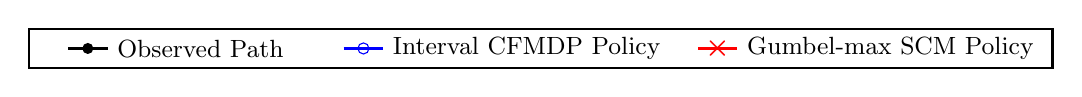
\begin{tikzpicture}[scale=1.0, every node/.style={scale=1.0}]
            \draw[thick, black] (-3, -0.25) rectangle (10, 0.25);
            %
            \draw[black, line width=1pt] (-2.5, 0.0) -- (-2,0.0);
            \fill[black] (-2.25,0.0) circle (2pt); %
            \node[right] at (-2,0.0) {\small Observed Path};
            
            %
            \draw[blue, line width=1pt] (1.0,0.0) -- (1.5,0.0);
            \node[draw=blue, circle, minimum size=4pt, inner sep=0pt] at (1.25,0.0) {}; %
            \node[right] at (1.5,0.0) {\small Interval CFMDP Policy};
            
            %
            \draw[red, line width=1pt] (5.5,0) -- (6,0);
            \node[red] at (5.75,0) {$\boldsymbol{\times}$}; %
            \node[right] at (6,0) {\small Gumbel-max SCM Policy};
        \end{tikzpicture}
    }\\
    %
    \subfigure[\footnotesize Lowest cumulative reward: Interval CFMDP ($312$), Gumbel-max SCM ($312$)]{%
        \resizebox{0.76\columnwidth}{!}{
             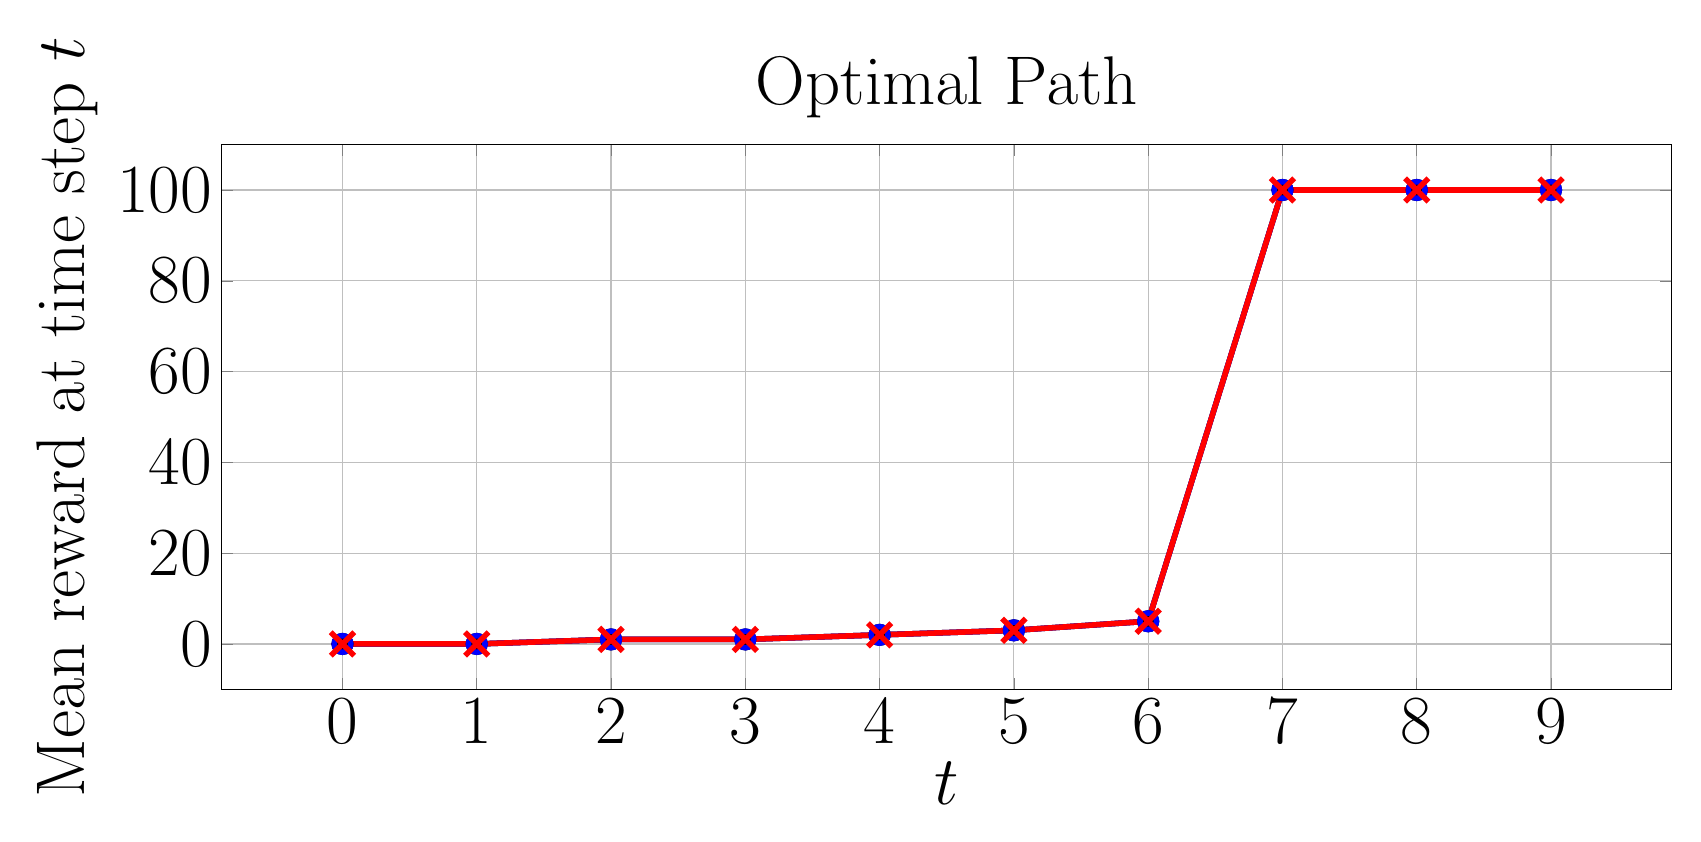
\begin{tikzpicture}
                \begin{axis}[
                    xlabel={$t$},
                    ylabel={Mean reward at time step $t$},
                    title={Optimal Path},
                    grid=both,
                    width=20cm, height=8.5cm,
                    every axis/.style={font=\Huge},
                    %
                ]
                \addplot[
                    color=black, %
                    mark=*, %
                    line width=2pt,
                    mark size=3pt,
                    error bars/.cd,
                    y dir=both, %
                    y explicit, %
                    error bar style={line width=1pt,solid},
                    error mark options={line width=1pt,mark size=4pt,rotate=90}
                ]
                coordinates {
                    (0, 0.0)  +- (0, 0.0)
                    (1, 0.0)  +- (0, 0.0) 
                    (2, 1.0)  +- (0, 0.0) 
                    (3, 1.0)  +- (0, 0.0)
                    (4, 2.0)  +- (0, 0.0)
                    (5, 3.0) +- (0, 0.0)
                    (6, 5.0) +- (0, 0.0)
                    (7, 100.0) +- (0, 0.0)
                    (8, 100.0) +- (0, 0.0)
                    (9, 100.0) +- (0, 0.0)
                };
                %
                \addplot[
                    color=blue, %
                    mark=o, %
                    line width=2pt,
                    mark size=3pt,
                    error bars/.cd,
                    y dir=both, %
                    y explicit, %
                    error bar style={line width=1pt,solid},
                    error mark options={line width=1pt,mark size=4pt,rotate=90}
                ]
                 coordinates {
                    (0, 0.0)  +- (0, 0.0)
                    (1, 0.0)  +- (0, 0.0) 
                    (2, 1.0)  +- (0, 0.0) 
                    (3, 1.0)  +- (0, 0.0)
                    (4, 2.0)  +- (0, 0.0)
                    (5, 3.0) +- (0, 0.0)
                    (6, 5.0) +- (0, 0.0)
                    (7, 100.0) +- (0, 0.0)
                    (8, 100.0) +- (0, 0.0)
                    (9, 100.0) +- (0, 0.0)
                };
                %
                \addplot[
                    color=red, %
                    mark=x, %
                    line width=2pt,
                    mark size=6pt,
                    error bars/.cd,
                    y dir=both, %
                    y explicit, %
                    error bar style={line width=1pt,solid},
                    error mark options={line width=1pt,mark size=4pt,rotate=90}
                ]
                coordinates {
                    (0, 0.0)  +- (0, 0.0)
                    (1, 0.0)  +- (0, 0.0) 
                    (2, 1.0)  +- (0, 0.0) 
                    (3, 1.0)  +- (0, 0.0)
                    (4, 2.0)  +- (0, 0.0)
                    (5, 3.0) +- (0, 0.0)
                    (6, 5.0) +- (0, 0.0)
                    (7, 100.0) +- (0, 0.0)
                    (8, 100.0) +- (0, 0.0)
                    (9, 100.0) +- (0, 0.0)
                };
                \end{axis}
            \end{tikzpicture}
         }
    }
    \hspace{1cm}
    \subfigure[\footnotesize Lowest cumulative reward: Interval CFMDP ($19$), Gumbel-max SCM ($-88$)]{%
         \resizebox{0.76\columnwidth}{!}{
            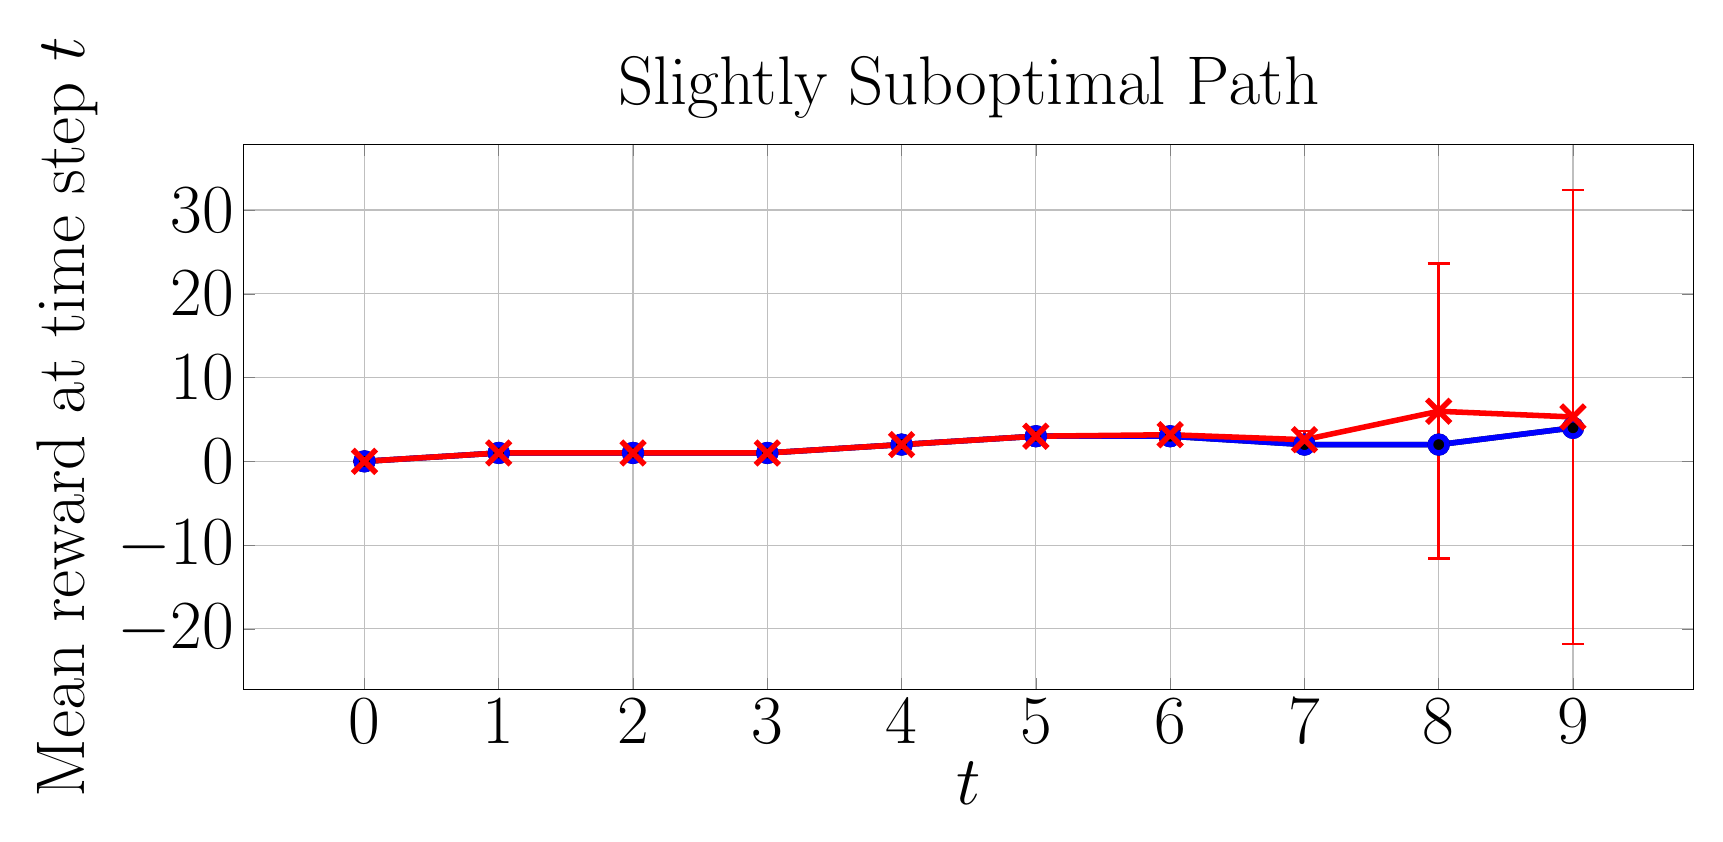
\begin{tikzpicture}
                \begin{axis}[
                    xlabel={$t$},
                    ylabel={Mean reward at time step $t$},
                    title={Slightly Suboptimal Path},
                    grid=both,
                    width=20cm, height=8.5cm,
                    every axis/.style={font=\Huge},
                    %
                ]
                \addplot[
                    color=black, %
                    mark=*, %
                    line width=2pt,
                    mark size=3pt,
                    error bars/.cd,
                    y dir=both, %
                    y explicit, %
                    error bar style={line width=1pt,solid},
                    error mark options={line width=1pt,mark size=4pt,rotate=90}
                ]
              coordinates {
                    (0, 0.0)  +- (0, 0.0)
                    (1, 1.0)  +- (0, 0.0) 
                    (2, 1.0)  +- (0, 0.0) 
                    (3, 1.0)  +- (0, 0.0)
                    (4, 2.0)  +- (0, 0.0)
                    (5, 3.0) +- (0, 0.0)
                    (6, 3.0) +- (0, 0.0)
                    (7, 2.0) +- (0, 0.0)
                    (8, 2.0) +- (0, 0.0)
                    (9, 4.0) +- (0, 0.0)
                };
                %
                \addplot[
                    color=blue, %
                    mark=o, %
                    line width=2pt,
                    mark size=3pt,
                    error bars/.cd,
                    y dir=both, %
                    y explicit, %
                    error bar style={line width=1pt,solid},
                    error mark options={line width=1pt,mark size=4pt,rotate=90}
                ]
              coordinates {
                    (0, 0.0)  +- (0, 0.0)
                    (1, 1.0)  +- (0, 0.0) 
                    (2, 1.0)  +- (0, 0.0) 
                    (3, 1.0)  +- (0, 0.0)
                    (4, 2.0)  +- (0, 0.0)
                    (5, 3.0) +- (0, 0.0)
                    (6, 3.0) +- (0, 0.0)
                    (7, 2.0) +- (0, 0.0)
                    (8, 2.0) +- (0, 0.0)
                    (9, 4.0) +- (0, 0.0)
                };
                %
                \addplot[
                    color=red, %
                    mark=x, %
                    line width=2pt,
                    mark size=6pt,
                    error bars/.cd,
                    y dir=both, %
                    y explicit, %
                    error bar style={line width=1pt,solid},
                    error mark options={line width=1pt,mark size=4pt,rotate=90}
                ]
                coordinates {
                    (0, 0.0)  +- (0, 0.0)
                    (1, 1.0)  +- (0, 0.0) 
                    (2, 1.0)  +- (0, 0.0) 
                    (3, 1.0)  +- (0, 0.0)
                    (4, 2.0)  += (0, 0.0)
                    (5, 3.0)  += (0, 0.0)
                    (6, 3.17847) += (0, 0.62606746) -= (0, 0.62606746)
                    (7, 2.5832885) += (0, 1.04598233) -= (0, 1.04598233)
                    (8, 5.978909) += (0, 17.60137623) -= (0, 17.60137623)
                    (9, 5.297059) += (0, 27.09227512) -= (0, 27.09227512)
                };
                \end{axis}
            \end{tikzpicture}
         }
    }\\[-1.5pt]
    \subfigure[\footnotesize Lowest cumulative reward: Interval CFMDP ($14$), Gumbel-max SCM ($-598$)]{%
         \resizebox{0.76\columnwidth}{!}{
             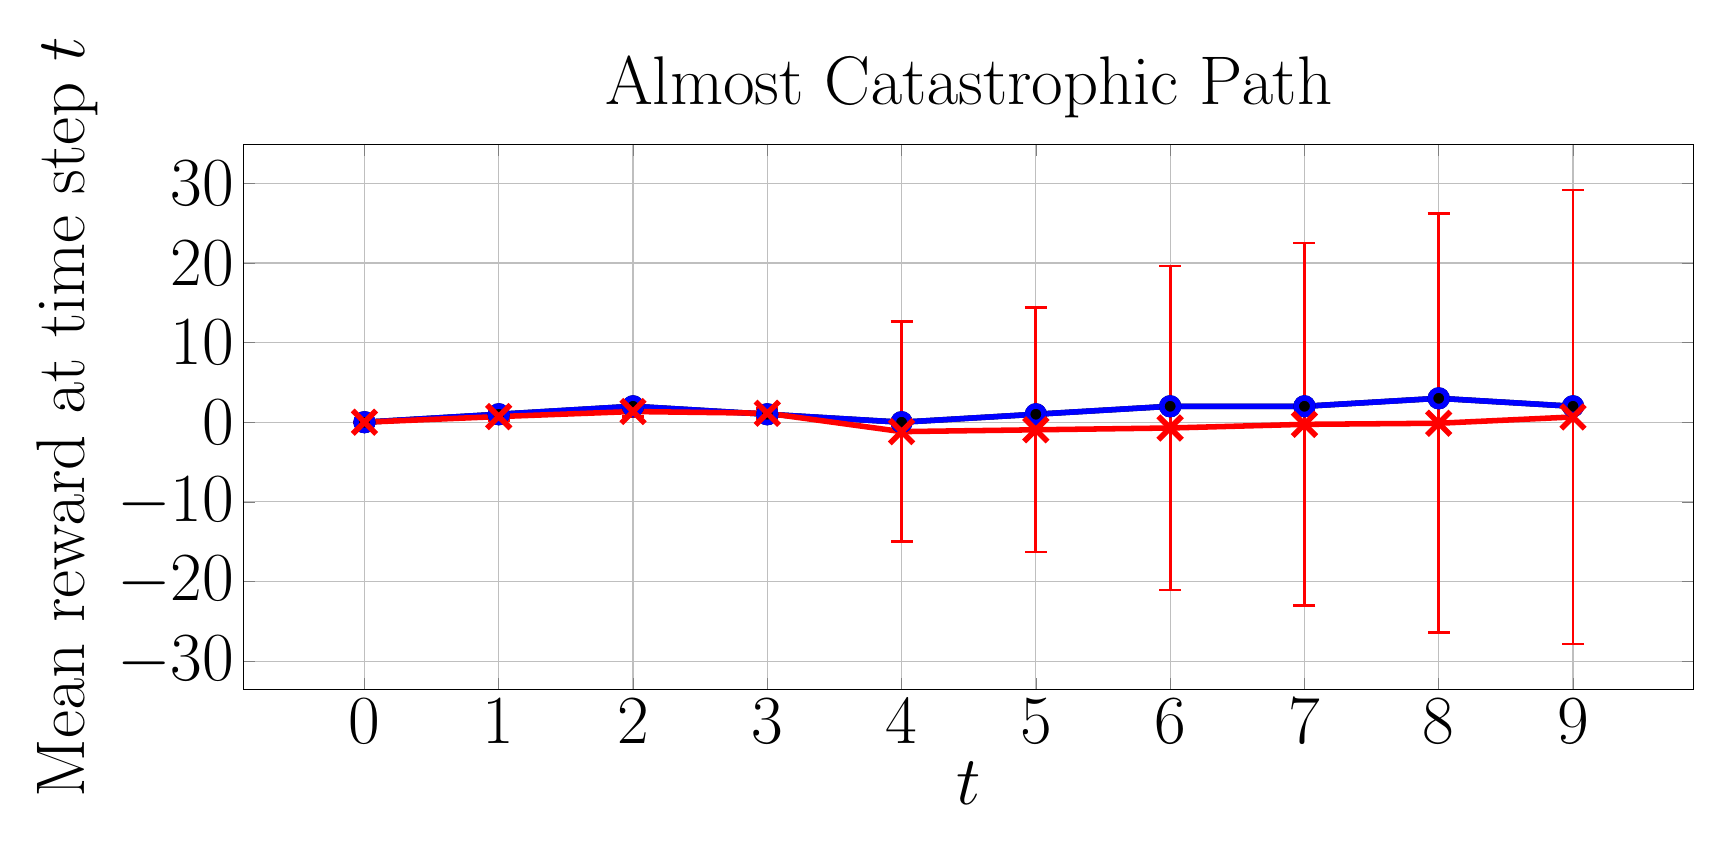
\begin{tikzpicture}
                \begin{axis}[
                    xlabel={$t$},
                    ylabel={Mean reward at time step $t$},
                    title={Almost Catastrophic Path},
                    grid=both,
                    width=20cm, height=8.5cm,
                    every axis/.style={font=\Huge},
                    %
                ]
                \addplot[
                    color=black, %
                    mark=*, %
                    line width=2pt,
                    mark size=3pt,
                    error bars/.cd,
                    y dir=both, %
                    y explicit, %
                    error bar style={line width=1pt,solid},
                    error mark options={line width=1pt,mark size=4pt,rotate=90}
                ]
                coordinates {
                    (0, 0.0)  +- (0, 0.0)
                    (1, 1.0)  +- (0, 0.0) 
                    (2, 2.0)  +- (0, 0.0) 
                    (3, 1.0)  +- (0, 0.0)
                    (4, 0.0)  +- (0, 0.0)
                    (5, 1.0) +- (0, 0.0)
                    (6, 2.0) +- (0, 0.0)
                    (7, 2.0) +- (0, 0.0)
                    (8, 3.0) +- (0, 0.0)
                    (9, 2.0) +- (0, 0.0)
                };
                %
                \addplot[
                    color=blue, %
                    mark=o, %
                    line width=2pt,
                    mark size=3pt,
                    error bars/.cd,
                    y dir=both, %
                    y explicit, %
                    error bar style={line width=1pt,solid},
                    error mark options={line width=1pt,mark size=4pt,rotate=90}
                ]
                coordinates {
                    (0, 0.0)  +- (0, 0.0)
                    (1, 1.0)  +- (0, 0.0) 
                    (2, 2.0)  +- (0, 0.0) 
                    (3, 1.0)  +- (0, 0.0)
                    (4, 0.0)  +- (0, 0.0)
                    (5, 1.0) +- (0, 0.0)
                    (6, 2.0) +- (0, 0.0)
                    (7, 2.0) +- (0, 0.0)
                    (8, 3.0) +- (0, 0.0)
                    (9, 2.0) +- (0, 0.0)
                };
                %
                \addplot[
                    color=red, %
                    mark=x, %
                    line width=2pt,
                    mark size=6pt,
                    error bars/.cd,
                    y dir=both, %
                    y explicit, %
                    error bar style={line width=1pt,solid},
                    error mark options={line width=1pt,mark size=4pt,rotate=90}
                ]
                coordinates {
                    (0, 0.0)  +- (0, 0.0)
                    (1, 0.7065655)  +- (0, 0.4553358) 
                    (2, 1.341673)  +- (0, 0.67091621) 
                    (3, 1.122926)  +- (0, 0.61281824)
                    (4, -1.1821935)  +- (0, 13.82444042)
                    (5, -0.952399)  +- (0, 15.35195457)
                    (6, -0.72672) +- (0, 20.33508414)
                    (7, -0.268983) +- (0, 22.77861454)
                    (8, -0.1310835) +- (0, 26.31013314)
                    (9, 0.65806) +- (0, 28.50670214)
                };
                %
            %
            %
            %
            %
            %
            %
            %
            %
            %
            %
            %
            %
            %
            %
            %
            %
            %
            %
                \end{axis}
            \end{tikzpicture}
         }
    }
    \hspace{1cm}
    \subfigure[\footnotesize Lowest cumulative reward: Interval CFMDP ($-698$), Gumbel-max SCM ($-698$)]{%
         \resizebox{0.76\columnwidth}{!}{
            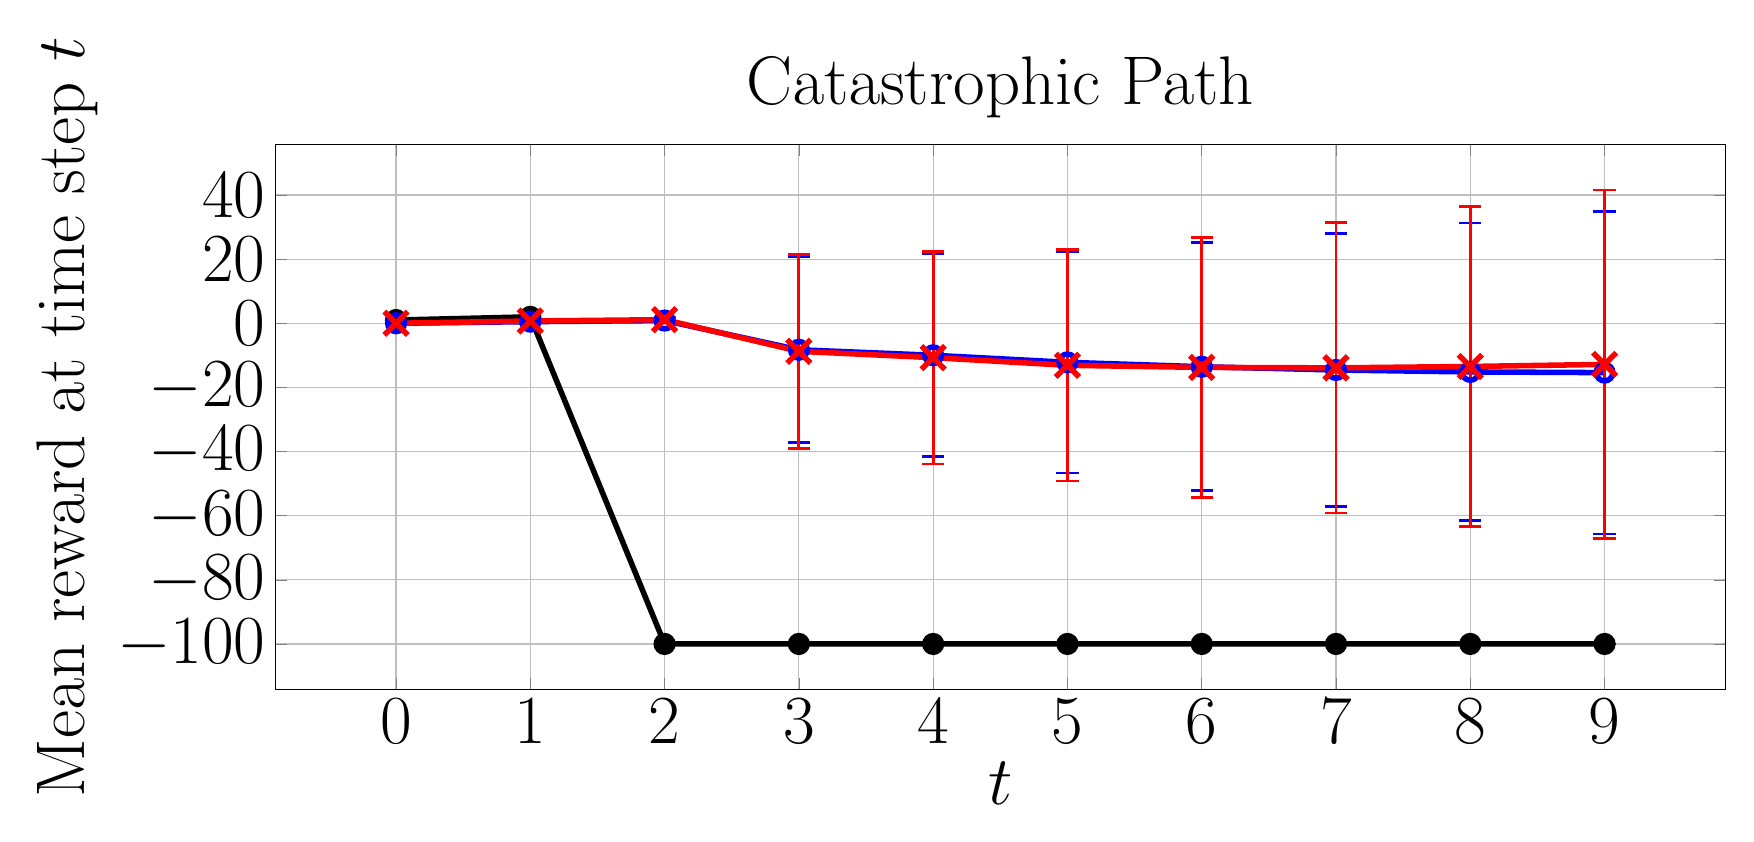
\begin{tikzpicture}
                \begin{axis}[
                    xlabel={$t$},
                    ylabel={Mean reward at time step $t$},
                    title={Catastrophic Path},
                    grid=both,
                    width=20cm, height=8.5cm,
                    every axis/.style={font=\Huge},
                    %
                ]
                \addplot[
                    color=black, %
                    mark=*, %
                    line width=2pt,
                    mark size=3pt,
                    error bars/.cd,
                    y dir=both, %
                    y explicit, %
                    error bar style={line width=1pt,solid},
                    error mark options={line width=1pt,mark size=4pt,rotate=90}
                ]
                coordinates {
                    (0, 1.0)  +- (0, 0.0)
                    (1, 2.0)  +- (0, 0.0) 
                    (2, -100.0)  +- (0, 0.0) 
                    (3, -100.0)  +- (0, 0.0)
                    (4, -100.0)  +- (0, 0.0)
                    (5, -100.0) +- (0, 0.0)
                    (6, -100.0) +- (0, 0.0)
                    (7, -100.0) +- (0, 0.0)
                    (8, -100.0) +- (0, 0.0)
                    (9, -100.0) +- (0, 0.0)
                };
                %
                \addplot[
                    color=blue, %
                    mark=o, %
                    line width=2pt,
                    mark size=3pt,
                    error bars/.cd,
                    y dir=both, %
                    y explicit, %
                    error bar style={line width=1pt,solid},
                    error mark options={line width=1pt,mark size=4pt,rotate=90}
                ]
                coordinates {
                    (0, 0.0)  +- (0, 0.0)
                    (1, 0.504814)  +- (0, 0.49997682) 
                    (2, 0.8439835)  +- (0, 0.76831917) 
                    (3, -8.2709165)  +- (0, 28.93656754)
                    (4, -9.981082)  +- (0, 31.66825363)
                    (5, -12.1776325) +- (0, 34.53463233)
                    (6, -13.556076) +- (0, 38.62845372)
                    (7, -14.574418) +- (0, 42.49603359)
                    (8, -15.1757075) +- (0, 46.41913968)
                    (9, -15.3900395) +- (0, 50.33563368)
                };
                %
                \addplot[
                    color=red, %
                    mark=x, %
                    line width=2pt,
                    mark size=6pt,
                    error bars/.cd,
                    y dir=both, %
                    y explicit, %
                    error bar style={line width=1pt,solid},
                    error mark options={line width=1pt,mark size=4pt,rotate=90}
                ]
                coordinates {
                    (0, 0.0)  +- (0, 0.0)
                    (1, 0.701873)  +- (0, 0.45743556) 
                    (2, 1.1227805)  +- (0, 0.73433129) 
                    (3, -8.7503255)  +- (0, 30.30257976)
                    (4, -10.722092)  +- (0, 33.17618589)
                    (5, -13.10721)  +- (0, 36.0648089)
                    (6, -13.7631645) +- (0, 40.56553451)
                    (7, -13.909043) +- (0, 45.23829402)
                    (8, -13.472517) +- (0, 49.96270296)
                    (9, -12.8278835) +- (0, 54.38618735)
                };
                %
            %
            %
            %
            %
            %
            %
            %
            %
            %
            %
            %
            %
            %
            %
            %
            %
            %
            %
                \end{axis}
            \end{tikzpicture}
         }
    }
    \caption{Average instant reward of CF paths induced by policies on GridWorld $p=0.4$.}
    \label{fig: reward p=0.4}
\end{figure*}

\subsection{Experimental Setup}
To compare policy performance, we measure the average rewards of counterfactual paths induced by our policy and the Gumbel-max policy by uniformly sampling $200$ counterfactual MDPs from the ICFMDP and generating $10,000$ counterfactual paths over each sampled CFMDP. \jl{Since the interval CFMDP depends on the observed path, we select $4$  paths of varying optimality to evaluate how the observed path impacts the performance of both policies: an optimal path, a slightly suboptimal path that could reach the optimal reward with a few changes, a catastrophic path that enters a catastrophic, terminal state with low reward, and an almost catastrophic path that was close to entering a catastrophic state.} When measuring the average probability bound widths and execution time needed to generate the ICFMDPs, we averaged over $20$ randomly generated observed paths
\footnote{Further training details are provided in Appendix \ref{app: training details}, and the code is provided at \href{https://github.com/ddv-lab/robust-cf-inference-in-MDPs}{https://github.com/ddv-lab/robust-cf-inference-in-MDPs}
%
%
.}.

\subsection{GridWorld}
\jl{The GridWorld MDP is a $4 \times 4$ grid where an agent must navigate from the top-left corner to the goal state in the bottom-right corner, avoiding a dangerous terminal state in the centre. At each time step, the agent can move up, down, left, or right, but there is a small probability (controlled by hyper-parameter $p$) of moving in an unintended direction. As the agent nears the goal, the reward for each state increases, culminating in a reward of $+100$ for reaching the goal. Entering the dangerous state results in a penalty of $-100$. We use two versions of GridWorld: a less stochastic version with $p=0.9$ (i.e., $90$\% chance of moving in the chosen direction) and a more stochastic version with $p=0.4$.}

\paragraph{GridWorld ($p=0.9$)}
When $p=0.9$, the counterfactual probability bounds are typically narrow (see Table \ref{tab:nonzero_probs} for average measurements). Consequently, as shown in Figure \ref{fig: reward p=0.9}, both policies are nearly identical and perform similarly well across the optimal, slightly suboptimal, and catastrophic paths.
%
However, for the almost catastrophic path, the interval CFMDP path is more conservative and follows the observed path more closely (as this is where the probability bounds are narrowest), which typically requires one additional step to reach the goal state than the Gumbel-max SCM policy.
%

\paragraph{GridWorld ($p=0.4$)}
\jl{When $p=0.4$, the GridWorld environment becomes more uncertain, increasing the risk of entering the dangerous state even if correct actions are chosen. Thus, as shown in Figure \ref{fig: reward p=0.4}, the interval CFMDP policy adopts a more conservative approach, avoiding deviation from the observed policy if it cannot guarantee higher counterfactual rewards (see the slightly suboptimal and almost catastrophic paths), whereas the Gumbel-max SCM is inconsistent: it can yield higher rewards, but also much lower rewards, reflected in the wide error bars.} For the catastrophic path, both policies must deviate from the observed path to achieve a higher reward and, in this case, perform similarly.
%
%
%
%
\subsection{Sepsis}
The Sepsis MDP \citep{oberst2019counterfactual} simulates trajectories of Sepsis patients. Each state consists of four vital signs (heart rate, blood pressure, oxygen concentration, and glucose levels), categorised as low, normal, or high.
and three treatments that can be toggled on/off at each time step (8 actions in total). Unlike \citet{oberst2019counterfactual}, we scale rewards based on the number of out-of-range vital signs, between $-1000$ (patient dies) and $1000$ (patient discharged). \jl{Like the GridWorld $p=0.4$ experiment, the Sepsis MDP is highly uncertain, as many states are equally likely to lead to optimal and poor outcomes. Thus, as shown in Figure \ref{fig: reward sepsis}, both policies follow the observed optimal and almost catastrophic paths to guarantee rewards are no worse than the observation.} However, improving the catastrophic path requires deviating from the observation. Here, the Gumbel-max SCM policy, on average, performs better than the interval CFMDP policy. But, since both policies have lower bounds clipped at $-1000$, neither policy reliably improves over the observation. In contrast, for the slightly suboptimal path, the interval CFMDP policy performs significantly better, shown by its higher lower bounds. 
Moreover, in these two cases, the worst-case counterfactual path generated by the interval CFMDP policy is better than that of the Gumbel-max SCM policy,
indicating its greater robustness.
%
\begin{figure*}
    \centering
     \resizebox{0.6\textwidth}{!}{
        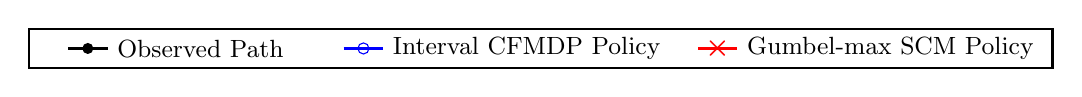
\begin{tikzpicture}[scale=1.0, every node/.style={scale=1.0}]
            \draw[thick, black] (-3, -0.25) rectangle (10, 0.25);
            %
            \draw[black, line width=1pt] (-2.5, 0.0) -- (-2,0.0);
            \fill[black] (-2.25,0.0) circle (2pt); %
            \node[right] at (-2,0.0) {\small Observed Path};
            
            %
            \draw[blue, line width=1pt] (1.0,0.0) -- (1.5,0.0);
            \node[draw=blue, circle, minimum size=4pt, inner sep=0pt] at (1.25,0.0) {}; %
            \node[right] at (1.5,0.0) {\small Interval CFMDP Policy};
            
            %
            \draw[red, line width=1pt] (5.5,0) -- (6,0);
            \node[red] at (5.75,0) {$\boldsymbol{\times}$}; %
            \node[right] at (6,0) {\small Gumbel-max SCM Policy};
        \end{tikzpicture}
    }\\
    \subfigure[\footnotesize Lowest cumulative reward: Interval CFMDP ($8000$), Gumbel-max SCM ($8000$)]{%
         \resizebox{0.76\columnwidth}{!}{
             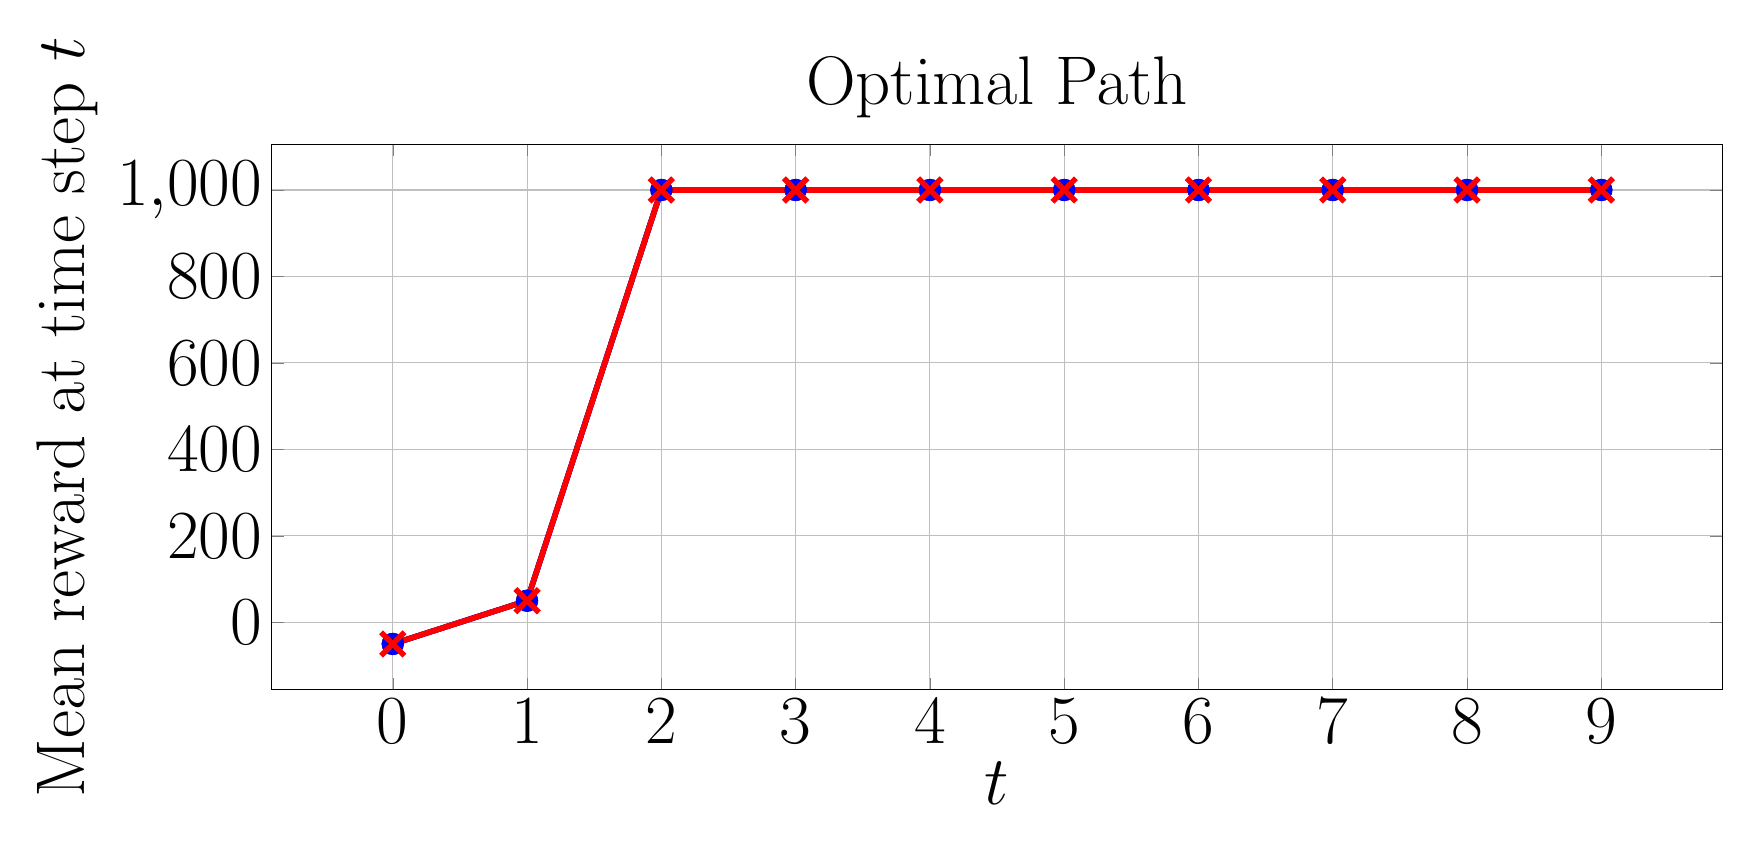
\begin{tikzpicture}
                \begin{axis}[
                    xlabel={$t$},
                    ylabel={Mean reward at time step $t$},
                    title={Optimal Path},
                    grid=both,
                    width=20cm, height=8.5cm,
                    every axis/.style={font=\Huge},
                    %
                ]
                \addplot[
                    color=black, %
                    mark=*, %
                    line width=2pt,
                    mark size=3pt,
                ]
                coordinates {
                    (0, -50.0)
                    (1, 50.0)
                    (2, 1000.0)
                    (3, 1000.0)
                    (4, 1000.0)
                    (5, 1000.0)
                    (6, 1000.0)
                    (7, 1000.0)
                    (8, 1000.0)
                    (9, 1000.0)
                };
                %
                \addplot[
                    color=blue, %
                    mark=o, %
                    line width=2pt,
                    mark size=3pt,
                    error bars/.cd,
                    y dir=both, %
                    y explicit, %
                    error bar style={line width=1pt,solid},
                    error mark options={line width=1pt,mark size=4pt,rotate=90}
                ]
                coordinates {
                    (0, -50.0)  +- (0, 0.0)
                    (1, 50.0)  +- (0, 0.0) 
                    (2, 1000.0)  +- (0, 0.0) 
                    (3, 1000.0)  +- (0, 0.0)
                    (4, 1000.0)  +- (0, 0.0)
                    (5, 1000.0) +- (0, 0.0)
                    (6, 1000.0) +- (0, 0.0)
                    (7, 1000.0) +- (0, 0.0)
                    (8, 1000.0) +- (0, 0.0)
                    (9, 1000.0) +- (0, 0.0)
                };
                %
                \addplot[
                    color=red, %
                    mark=x, %
                    line width=2pt,
                    mark size=6pt,
                    error bars/.cd,
                    y dir=both, %
                    y explicit, %
                    error bar style={line width=1pt,solid},
                    error mark options={line width=1pt,mark size=4pt,rotate=90}
                ]
                coordinates {
                    (0, -50.0)  +- (0, 0.0)
                    (1, 50.0)  +- (0, 0.0) 
                    (2, 1000.0)  +- (0, 0.0) 
                    (3, 1000.0)  +- (0, 0.0)
                    (4, 1000.0)  +- (0, 0.0)
                    (5, 1000.0) +- (0, 0.0)
                    (6, 1000.0) +- (0, 0.0)
                    (7, 1000.0) +- (0, 0.0)
                    (8, 1000.0) +- (0, 0.0)
                    (9, 1000.0) +- (0, 0.0)
                };
                %
                \end{axis}
            \end{tikzpicture}
         }
    }
    \hspace{1cm}
    \subfigure[\footnotesize Lowest cumulative reward: Interval CFMDP ($-5980$), Gumbel-max SCM ($-8000$)]{%
         \resizebox{0.76\columnwidth}{!}{
            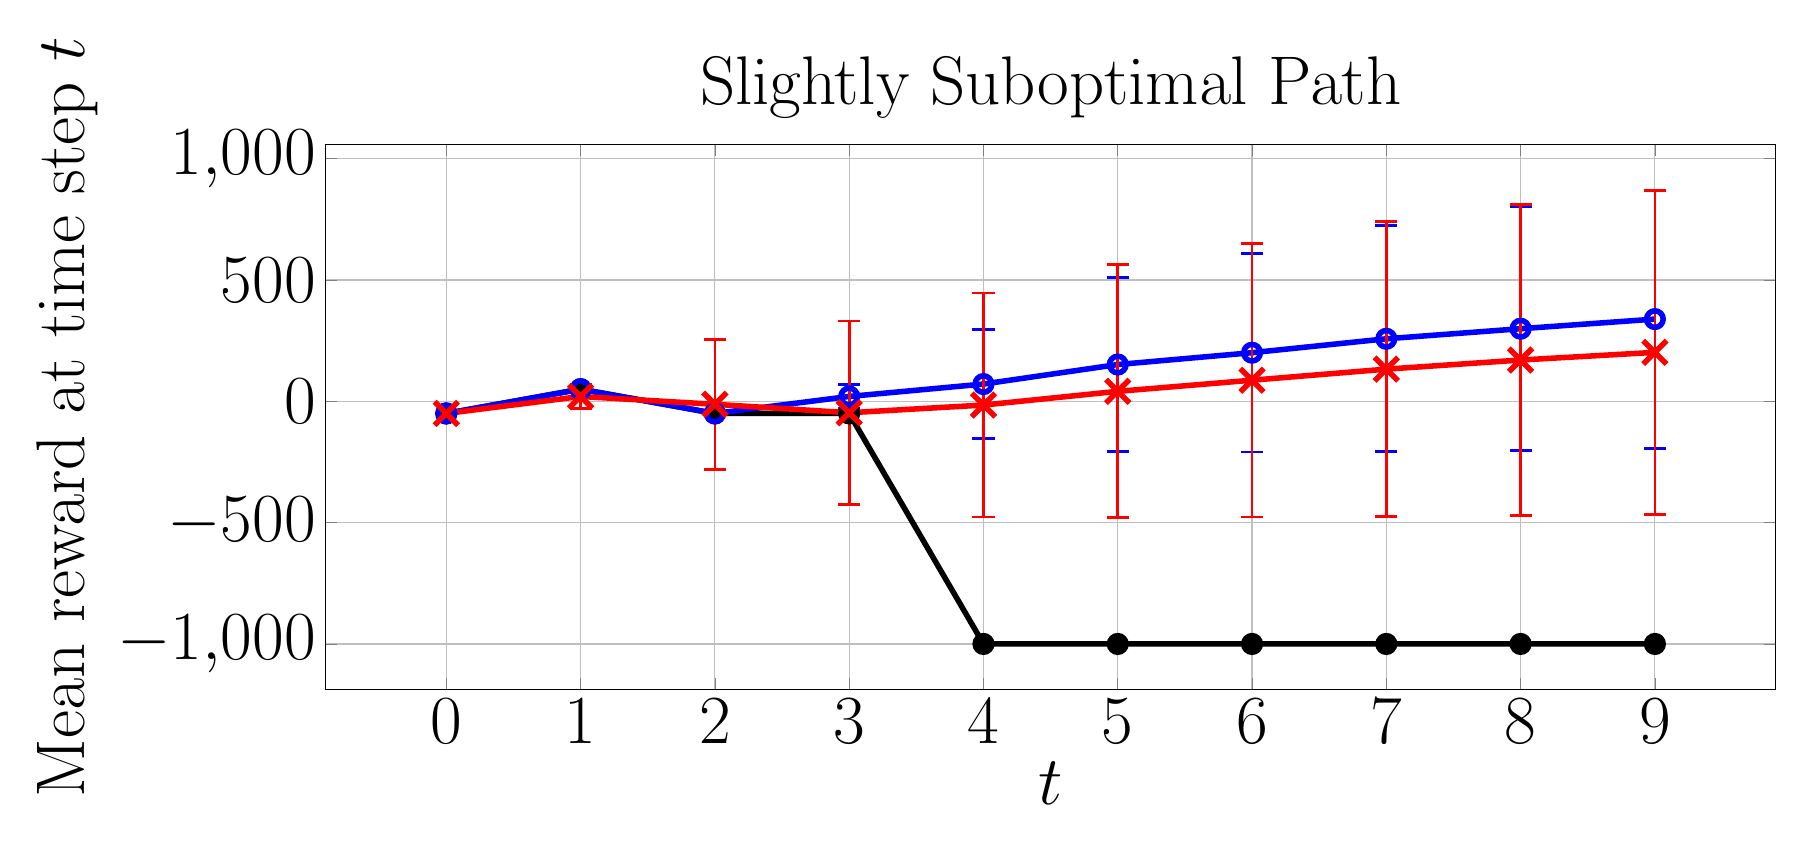
\begin{tikzpicture}
                \begin{axis}[
                    xlabel={$t$},
                    ylabel={Mean reward at time step $t$},
                    title={Slightly Suboptimal Path},
                    grid=both,
                    width=20cm, height=8.5cm,
                    every axis/.style={font=\Huge},
                    %
                ]
               \addplot[
                    color=black, %
                    mark=*, %
                    line width=2pt,
                    mark size=3pt,
                ]
                coordinates {
                    (0, -50.0)
                    (1, 50.0)
                    (2, -50.0)
                    (3, -50.0)
                    (4, -1000.0)
                    (5, -1000.0)
                    (6, -1000.0)
                    (7, -1000.0)
                    (8, -1000.0)
                    (9, -1000.0)
                };
                %
                \addplot[
                    color=blue, %
                    mark=o, %
                    line width=2pt,
                    mark size=3pt,
                    error bars/.cd,
                    y dir=both, %
                    y explicit, %
                    error bar style={line width=1pt,solid},
                    error mark options={line width=1pt,mark size=4pt,rotate=90}
                ]
                coordinates {
                    (0, -50.0)  +- (0, 0.0)
                    (1, 50.0)  +- (0, 0.0) 
                    (2, -50.0)  +- (0, 0.0) 
                    (3, 20.0631)  +- (0, 49.97539413)
                    (4, 71.206585)  +- (0, 226.02033693)
                    (5, 151.60797) +- (0, 359.23292559)
                    (6, 200.40593) +- (0, 408.86185176)
                    (7, 257.77948) +- (0, 466.10372804)
                    (8, 299.237465) +- (0, 501.82579506)
                    (9, 338.9129) +- (0, 532.06124996)
                };
                %
                \addplot[
                    color=red, %
                    mark=x, %
                    line width=2pt,
                    mark size=6pt,
                    error bars/.cd,
                    y dir=both, %
                    y explicit, %
                    error bar style={line width=1pt,solid},
                    error mark options={line width=1pt,mark size=4pt,rotate=90}
                ]
                coordinates {
                    (0, -50.0)  +- (0, 0.0)
                    (1, 20.00736)  +- (0, 49.99786741) 
                    (2, -12.282865)  +- (0, 267.598755) 
                    (3, -47.125995)  +- (0, 378.41755832)
                    (4, -15.381965)  +- (0, 461.77616558)
                    (5, 41.15459) +- (0, 521.53189262)
                    (6, 87.01595) +- (0, 564.22243126 )
                    (7, 132.62376) +- (0, 607.31338037)
                    (8, 170.168145) +- (0, 641.48013693)
                    (9, 201.813135) +- (0, 667.29441777)
                };
                %
                %
                %
                %
                %
                %
                %
                %
                %
                %
                %
                %
                %
                %
                %
                %
                %
                %
                %
                \end{axis}
            \end{tikzpicture}
         }
    }\\[-1.5pt]
    \subfigure[\footnotesize Lowest cumulative reward: Interval CFMDP ($100$), Gumbel-max SCM ($100$)]{%
         \resizebox{0.76\columnwidth}{!}{
             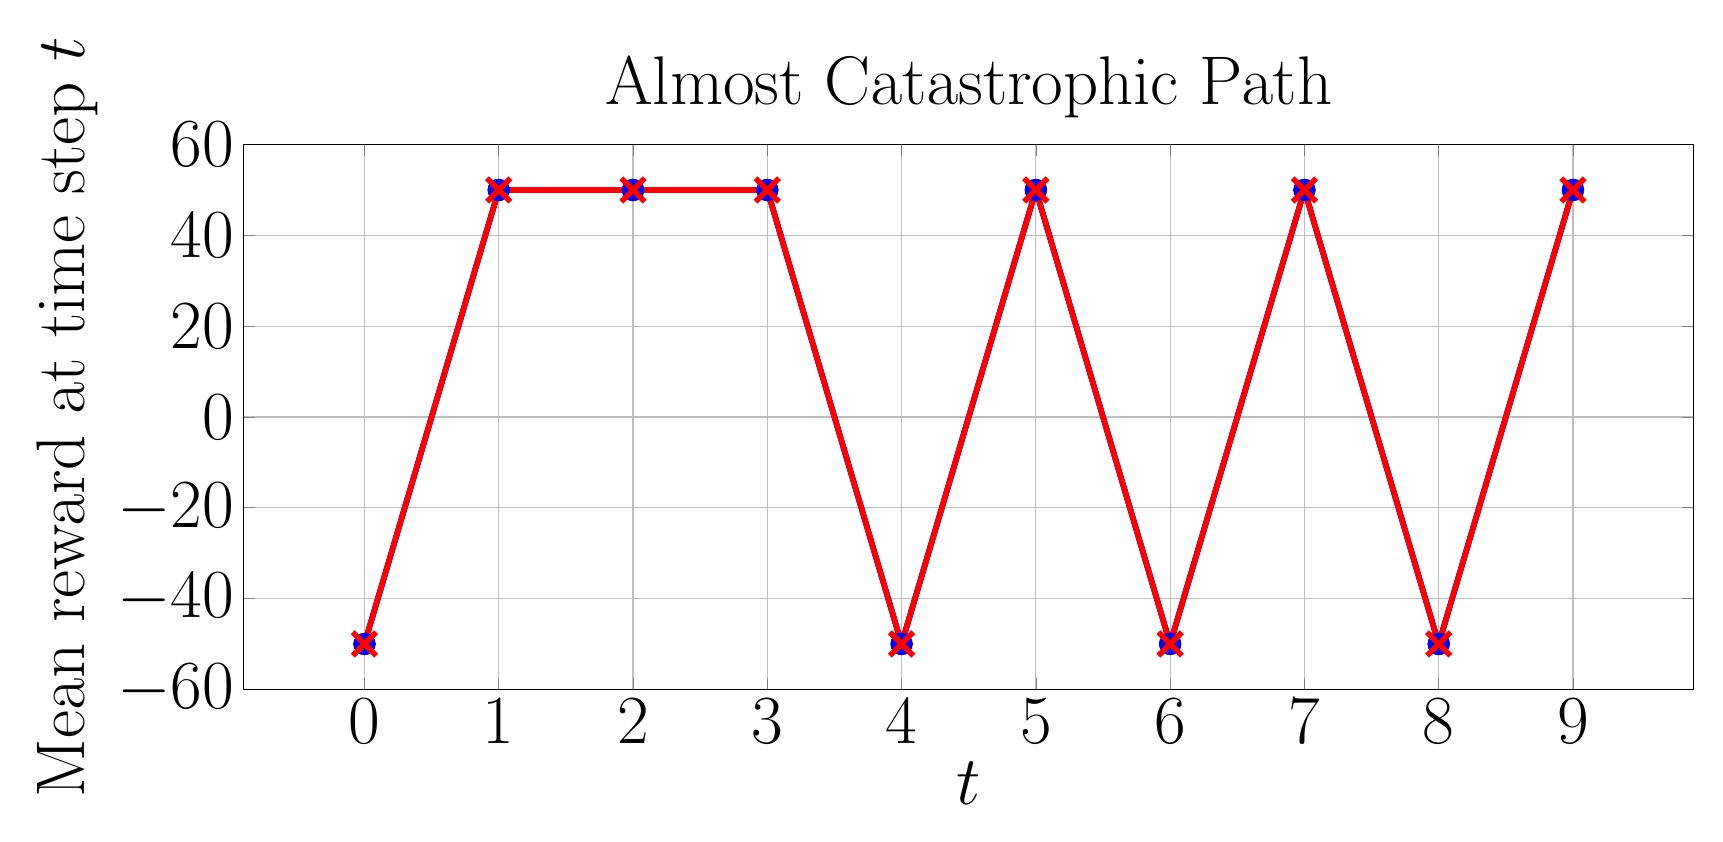
\begin{tikzpicture}
                \begin{axis}[
                    xlabel={$t$},
                    ylabel={Mean reward at time step $t$},
                    title={Almost Catastrophic Path},
                    grid=both,
                    every axis/.style={font=\Huge},
                    width=20cm, height=8.5cm,
                    %
                ]
               \addplot[
                    color=black, %
                    mark=*, %
                    line width=2pt,
                    mark size=3pt,
                ]
                coordinates {
                    (0, -50.0)
                    (1, 50.0)
                    (2, 50.0)
                    (3, 50.0)
                    (4, -50.0)
                    (5, 50.0)
                    (6, -50.0)
                    (7, 50.0)
                    (8, -50.0)
                    (9, 50.0)
                };
                %
                %
                \addplot[
                    color=blue, %
                    mark=o, %
                    line width=2pt,
                    mark size=3pt,
                    error bars/.cd,
                    y dir=both, %
                    y explicit, %
                    error bar style={line width=1pt,solid},
                    error mark options={line width=1pt,mark size=4pt,rotate=90}
                ]
                coordinates {
                    (0, -50.0)  +- (0, 0.0)
                    (1, 50.0)  +- (0, 0.0) 
                    (2, 50.0)  +- (0, 0.0) 
                    (3, 50.0)  +- (0, 0.0)
                    (4, -50.0)  +- (0, 0.0)
                    (5, 50.0) +- (0, 0.0)
                    (6, -50.0) +- (0, 0.0)
                    (7, 50.0) +- (0, 0.0)
                    (8, -50.0) +- (0, 0.0)
                    (9, 50.0) +- (0, 0.0)
                };
                %
                \addplot[
                    color=red, %
                    mark=x, %
                    line width=2pt,
                    mark size=6pt,
                    error bars/.cd,
                    y dir=both, %
                    y explicit, %
                    error bar style={line width=1pt,solid},
                    error mark options={line width=1pt,mark size=4pt,rotate=90}
                ]
                coordinates {
                    (0, -50.0)  +- (0, 0.0)
                    (1, 50.0)  +- (0, 0.0) 
                    (2, 50.0)  +- (0, 0.0) 
                    (3, 50.0)  +- (0, 0.0)
                    (4, -50.0)  +- (0, 0.0)
                    (5, 50.0) +- (0, 0.0)
                    (6, -50.0) +- (0, 0.0)
                    (7, 50.0) +- (0, 0.0)
                    (8, -50.0) +- (0, 0.0)
                    (9, 50.0) +- (0, 0.0)
                };
                %
                %
                %
                %
                %
                %
                %
                %
                %
                %
                %
                %
                %
                %
                %
                %
                %
                %
                %
                \end{axis}
            \end{tikzpicture}
         }
    }
    \hspace{1cm}
    \subfigure[\footnotesize Lowest cumulative reward: Interval CFMDP ($-7150$), Gumbel-max SCM ($-9050$)]{%
         \resizebox{0.76\columnwidth}{!}{
            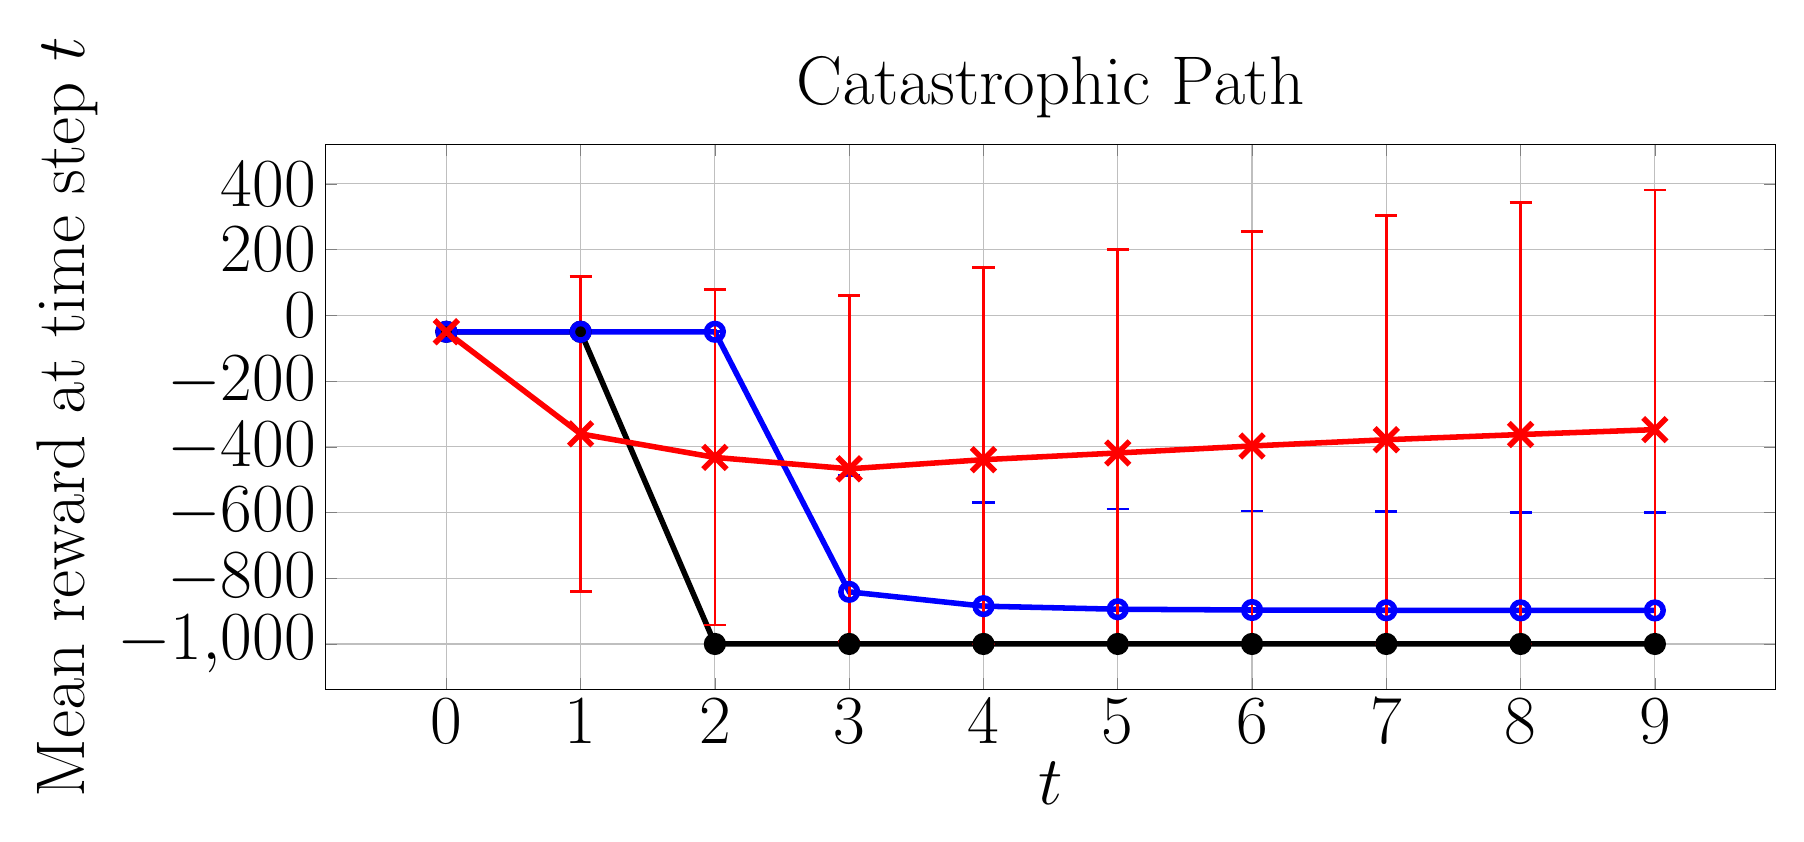
\begin{tikzpicture}
                \begin{axis}[
                    xlabel={$t$},
                    ylabel={Mean reward at time step $t$},
                    title={Catastrophic Path},
                    grid=both,
                    width=20cm, height=8.5cm,
                    every axis/.style={font=\Huge},
                    %
                ]
               \addplot[
                    color=black, %
                    mark=*, %
                    line width=2pt,
                    mark size=3pt,
                ]
                coordinates {
                    (0, -50.0)
                    (1, -50.0)
                    (2, -1000.0)
                    (3, -1000.0)
                    (4, -1000.0)
                    (5, -1000.0)
                    (6, -1000.0)
                    (7, -1000.0)
                    (8, -1000.0)
                    (9, -1000.0)
                };
                %
                %
                \addplot[
                    color=blue, %
                    mark=o, %
                    line width=2pt,
                    mark size=3pt,
                    error bars/.cd,
                    y dir=both, %
                    y explicit, %
                    error bar style={line width=1pt,solid},
                    error mark options={line width=1pt,mark size=4pt,rotate=90}
                ]
                coordinates {
                    (0, -50.0)  +- (0, 0.0)
                    (1, -50.0)  +- (0, 0.0) 
                    (2, -50.0)  +- (0, 0.0) 
                    (3, -841.440725)  += (0, 354.24605512) -= (0, 158.559275)
                    (4, -884.98225)  += (0, 315.37519669) -= (0, 115.01775)
                    (5, -894.330425) += (0, 304.88572805) -= (0, 105.669575)
                    (6, -896.696175) += (0, 301.19954514) -= (0, 103.303825)
                    (7, -897.4635) += (0, 299.61791279) -= (0, 102.5365)
                    (8, -897.77595) += (0, 298.80392585) -= (0, 102.22405)
                    (9, -897.942975) += (0, 298.32920557) -= (0, 102.057025)
                };
                %
                \addplot[
                    color=red, %
                    mark=x, %
                    line width=2pt,
                    mark size=6pt,
                    error bars/.cd,
                    y dir=both, %
                    y explicit, %
                    error bar style={line width=1pt,solid},
                    error mark options={line width=1pt,mark size=4pt,rotate=90}
                ]
            coordinates {
                    (0, -50.0)  +- (0, 0.0)
                    (1, -360.675265)  +- (0, 479.39812699) 
                    (2, -432.27629)  +- (0, 510.38620897) 
                    (3, -467.029545)  += (0, 526.36009628) -= (0, 526.36009628)
                    (4, -439.17429)  += (0, 583.96638919) -= (0, 560.82571)
                    (5, -418.82704) += (0, 618.43027478) -= (0, 581.17296)
                    (6, -397.464895) += (0, 652.67322574) -= (0, 602.535105)
                    (7, -378.49052) += (0, 682.85407033) -= (0, 621.50948)
                    (8, -362.654195) += (0, 707.01412023) -= (0, 637.345805)
                    (9, -347.737935) += (0, 729.29076479) -= (0, 652.262065)
                };
                %
                %
                %
                %
                %
                %
                %
                %
                %
                %
                %
                %
                %
                %
                %
                %
                %
                %
                %
                \end{axis}
            \end{tikzpicture}
         }
    }
    \caption{Average instant reward of CF paths induced by policies on Sepsis.}
    \label{fig: reward sepsis}
\end{figure*}

%
%
%
\subsection{Interval CFMDP Bounds}
%
%
Table \ref{tab:nonzero_probs} presents the mean counterfactual probability bound widths (excluding transitions where the upper bound is $0$) for each MDP, averaged over 20 observed paths. We compare the bounds under counterfactual stability (CS) and monotonicity (M) assumptions, CS alone, and no assumptions. This shows that the assumptions marginally reduce the bound widths, indicating the assumptions tighten the bounds without excluding too many causal models, as intended.
\renewcommand{\arraystretch}{1}

\begin{table}
\centering
\caption{Mean width of counterfactual probability bounds}
\resizebox{0.8\columnwidth}{!}{%
\begin{tabular}{|c|c|c|c|}
\hline
\multirow{2}{*}{\textbf{Environment}} & \multicolumn{3}{c|}{\textbf{Assumptions}} \\ \cline{2-4}
 & \textbf{CS + M} & \textbf{CS} & \textbf{None\tablefootnote{\jl{Equivalent to \citet{li2024probabilities}'s bounds (see Section \ref{sec: equivalence with Li}).}}} \\ \hline
\textbf{GridWorld} ($p=0.9$) & 0.0817 & 0.0977 & 0.100 \\ \hline
\textbf{GridWorld} ($p=0.4$) & 0.552  & 0.638  & 0.646 \\ \hline
\textbf{Sepsis} & 0.138 & 0.140 & 0.140 \\ \hline
\end{tabular}
}
\label{tab:nonzero_probs}
\end{table}


\subsection{Execution Times}
Table \ref{tab: times} compares the average time needed to generate the interval CFMDP vs.\ the Gumbel-max SCM CFMDP for 20 observations.
The GridWorld algorithms were run single-threaded, while the Sepsis experiments were run in parallel.
Generating the interval CFMDP is significantly faster as it uses exact analytical bounds, whereas the Gumbel-max CFMDP requires sampling from the Gumbel distribution to estimate counterfactual transition probabilities. \jl{Since constructing the counterfactual MDP models is the main bottleneck in both approaches, ours is more efficient overall and suitable for larger MDPs.}
\begin{table}
\centering
\caption{Mean execution time to generate CFMDPs}
\resizebox{0.99\columnwidth}{!}{%
\begin{tabular}{|c|c|c|}
\hline
\multirow{2}{*}{\textbf{Environment}} & \multicolumn{2}{c|}{\textbf{Mean Execution Time (s)}} \\ \cline{2-3} 
                                      & \textbf{Interval CFMDP} & \textbf{Gumbel-max CFMDP} \\ \hline
\textbf{GridWorld ($p=0.9$) }                  & 0.261                   & 56.1                      \\ \hline
\textbf{GridWorld ($p=0.4$)  }                 & 0.336                   & 54.5                      \\ \hline
\textbf{Sepsis}                                 & 688                     & 2940                      \\ \hline
\end{tabular}%
}
\label{tab: times}
\end{table}

%

%%%%%%%%%%%%%%%%%%%%%%%%%%%%%%%%%%%%%%%%%%%%%%%%%%%%%%%%%%%%%%%%%%%%%%%%%%%%%%
%%%%%%%%%%%%%%%%%%%%%%%%%%%%%%%%%%%%%%%%%%%%%%%%%%%%%%%%%%%%%%%%%%%%%%%%%%%%%%
\newpage
\section{Long Term Allocation (ILP)} \label{sec:ILP_dummy}
We use an ILP to find the optimal resource allocation on a longer time frame.
\apnote{remove this whole section once we finalize the whole paper.}
\subsection{ILP Formulation}
The ILP will try to minimize the cost of resources whilst servicing all the low-latency workloads. It will take into account re-routing and having multiple kinds of GPUs.
\subsubsection{Input}
\begin{itemize}
    \item $l$: number of different models we will try to serve
    \item $r$: number of regions
    \item $g$: number of GPU architectures we have
    \item $C: [\texttt{int}]_{l\times r\times g}$: $C_{i, j, k}$ is the number of instances of model $i$ at region $j$ running on GPU architecture $k$
    \item $R: [\texttt{int}]_{l\times r}$: $R_{i, j}$ is the \textbf{TPS requested} for model $i$ at region $j$ 
    \item $\bar{\theta}: [\texttt{float}]_{l\times g}$: $\bar{\theta}_{i, k}$ is the TPS of model $i$ on GPU $k$
    \item $G: [\texttt{float}]_{g}$: $G_{k}$ is the cost of acquiring GPU $k$
    \item $s: [\texttt{float}]_{l\times G}$: $s_{i, k}$ is the cost of acquiring model $i$ on GPU $k$
\end{itemize}
\subsubsection{Decision Variable}
Our decision variable $\delta$ will have dimension $l\times r\times g$ where $\delta_{i,j,k}$ will decide the change in number of instances assigned to model $i$ at region $j$ running on GPU $k$. 
\subsubsection{Constraints}
\begin{itemize}
    \item The first constraint will be to not deallocate more models at a particular configuration than there exist: $$\delta_{i,j,k} \geq C_{i, j, k}$$
    \item Second, we should ensure that we have capacity to process all the low latency tokens: 
    $$\theta_{i} = \sum^{j}\sum^{k}(C_{i, j, k} + \delta_{i, j, k}) * \bar{\theta}_{i, k} \text{  }\forall\text{ 
 }i\in\{l\}$$
    $$\theta_{i} \leq \sum^{j}R_{i, j} \text{ 
 }\forall\text{  }i\in \{l\}$$ Because we want to consider re-routing, this condition only checks that for each model, we should have enough capacity over all regions
 \item Next, we want each region $j$ to process atleast $(1-\gamma)R_{i, j}$ and atmost $(1+\gamma)R_{i, j}$ of its tokens for model $i$ in order to limit routing:
 $$\hat{\theta}_{i, j} = \sum^{k}(C_{i, j, k} + \delta_{i, j, k}) * \bar{\theta}_{i, k}$$
 $$(1-\gamma)R_{i, j} \leq \hat{\theta}_{i, j} \text{  }\forall\text{  }(i, j)\in\{l\}\times \{r\}$$
\end{itemize}
\subsubsection{Objective}
Our objective is to minimize the cost for capacity for answering all queries. Cost is affected by allocating new GPUs as well as the start up time for each model. Similarly, it is reduced when you deallocate any GPUs, but the model does not impact that cost:
$$\texttt{GPU cost} = \sum^{k}((\sum^{i, j}\delta_{i, j, k}) * G_{k})$$
$$I_{i, j, k} = \max(0, \delta_{i, j, k})$$
$$\texttt{Model startup cost} = \sum^{k}\sum^{i}(\sum^{j}I_{i, j, k} * s_{i, k})$$
$$\min (\texttt{GPU cost} + \texttt{Model startup cost})$$
\subsection{Load Estimation}
We use ARIMA modelling for estimating the load
\subsection{Buffer Addition using NIW}
We add known non-interactive workloads to the estimated load as buffer
\subsection{Combining Proactive and Reactive Mechanisms}
The proactive mechanism will tell us the final state we should aim for. The reactive mechanism will help us guide there. It will try to converge to the proactive mechanism when there are bursts of requests.


% \section{Results}
\label{sec:Results}

In this section, we present various analysis results that demonstrate the adoption of code obfuscation in Google Play.

\subsection{Overall Obfuscation Trends} 
\label{sec:obstrend}

\subsubsection{Presence of obfuscation} Out of the 548,967 Google Play Store APKs analyzed, we identified 308,782 obfuscated apps, representing approximately 56.25\% of the total. In Figure~\ref{fig:obfuscated_percentage}, we show the year-wise percentage of obfuscated apps for 2016-2023. There is an overall obfuscation increase of 13\% between 2016 and 2023, and as can be seen, the percentage of obfuscated apps has been increasing in the last few years, barring 2019 and 2020. As explained in Section~\ref{subsec:dataset}, 2019 and 2020 contain apps that are more likely to be abandoned by developers, and as such, they may not use advanced development practices.

\begin{figure}[h!]
\centering
    \includegraphics[width=\linewidth]{Figures/Only_obfuscation_trendV2.pdf}
    \caption{Percentage of obfuscated apps by year} \vspace{-4mm}
    \label{fig:obfuscated_percentage}
\end{figure}


From 2016 to 2018, the obfuscation levels were relatively stable at around 50-55\%, while from 2021 to 2023, there was a marked rise, reaching approximately 66\% in 2023. This indicates a growing focus on app protection measures among developers, likely driven by heightened security and IP concerns and the availability of advanced obfuscation tools.


\subsubsection{Obfuscation tools} Among the obfuscated APKs, our tool detector identified that 40.92\% of the apps use Proguard, 36.64\% use Allatori, 1.01\% use DashO, and 21.43\% use other (i.e., unknown) tools. We show the yearly trends in Figure~\ref{fig:ofbuscated_tool}. Note that we omit results in 2019 and 2020 ({\bf cf.} Section~\ref{subsec:dataset}).

ProGuard and Allatori are the most consistently used obfuscation tools, with ProGuard showing a slight overall increase in popularity and Allatori demonstrating variability. This inclination could be attributed to ProGuard being the default obfuscator integrated into Android Studio, a widely used development environment for Android applications. Notably, ProGuard usage increased by 13\% from 2018 to 2021, likely due to the introduction of R8 in April 2019~\cite{release_note_android}, which further simplified ProGuard integration with Android apps.

\begin{figure}[h]
\centering
    \includegraphics[width=\linewidth]{Figures/Initial_Tool_Trend_2019_dropV2.pdf} 
    \caption{Yearly obfuscation tool usage}
    \label{fig:ofbuscated_tool}
\end{figure}


DashO consistently remains low in usage, likely due to its high cost. The use of other obfuscation tools decreased until 2018 but has shown a resurgence from 2021 to 2023. This suggests that developers might be using other or custom tools, or our detector might be predicting some apps obfuscated with Proguard or Allatori as `other.' To investigate, we manually checked a sample of apps from the `other' category and confirmed they are indeed obfuscated. However, we could not determine which obfuscation tools the developers used. We discuss this potential limitation further in Section~\ref{sec:limitations}.


\subsubsection{Obfuscation techniques} We show the year-wise breakdown of obfuscation technique usage in Figure~\ref{fig:obfuscated_tech}. Among the various obfuscation techniques, Identifier Renaming emerged as the most prevalent, with 99.62\% of obfuscated apps using it alone or in combination with other methods (Categories of Only IR, IR and CF, IR and SE, or All three). Furthermore, 81.04\% of obfuscated apps used Control Flow Modification, and 62.76\% used String Encryption. The pervasive use of Identifier Renaming (IR) can be attributed to the fact that all obfuscation tools support it ({\bf cf.} Table~\ref{tab:ob_tool_cap}). Similarly, lower adoption of Control Flow Modification and String Encryption can be attributed to Proguard not supporting it. 

\begin{figure}[h]
\centering
    \includegraphics[width=\linewidth]{Figures/Initial_Tech_Trend_2019_dropV2.pdf} 
    \caption{Yearly obfuscation technique usage}
    \label{fig:obfuscated_tech}
\end{figure}



Next, we investigate the adoption of obfuscation on Google Play Store from various perspectives. Same as earlier, due to the smaller dataset size and possible bias ({\bf cf.} Section~\ref{subsec:dataset}), we exclude the APKs from 2019 and 2020 from this analyses.


\subsection{App Genre}
\label{sec:app_genre}

First, we investigate whether the obfuscation practices vary according to the App genre. Initially, we analysed all the APKs together before separating them into two snapshots.


\begin{figure*}[h]
    \centering
    \includegraphics[width=\linewidth]{Figures/AppGenreObfuscationV3.pdf}
    \caption{Obfuscated app percentage by genre (overall)}
    \label{fig:app_genre_overall}
\end{figure*}

Figure~\ref{fig:app_genre_overall} shows the genre-wise obfuscated app percentage. We note that 19 genres have more than 60\% of the apps obfuscated, and almost all the genres have more than 40\% obfuscation percentage. \textit{Casino} genre has the highest obfuscation percentage rate at 80\%, and overall, game genres tend to be more obfuscated than the other genres. The higher obfuscation usage in casino apps is logical due to their nature. These apps often simulate or involve gambling activities and handle monetary transactions and sensitive data related to in-game purchases, making them attractive targets for reverse engineering and hacking. This necessitates robust security measures to prevent fraud and protect user data. 


\begin{figure}[h]
    \centering
    \includegraphics[width=\linewidth]{Figures/AppGenre2018_2023ComparisonV3.pdf}
    \caption{Percentage of obfuscated apps by genre (2018-2023)}
    \label{fig:app_genre_comparison}
\end{figure}



\subsubsection{Genre-wise obfuscation trends in the two snapshots} To investigate the adoption of obfuscation over time, we study the two snapshots of Google Play separately, i.e., APKs from 2016-2018 as one group and APKs from 2021-2023 as another. 

Figure~\ref{fig:app_genre_comparison} illustrates the change in obfuscation levels by app genre between 2016-2018 to 2021-2023. Notably, app categories such as Education, Weather, and Parenting, which had obfuscation levels below the 2018 average, have increased to above the 2023 average by 2023. One possible reason for this in Education and Parenting apps can be the increase in online education activities during and after COVID-19 and the developers identifying the need for app hardening.

There are some genres, such as Casino and Action, for which the percentage of obfuscated apps didn't change across the two snapshots (i.e., purple and orange circles are close together in Figure~\ref{fig:app_genre_comparison}). This is because these genres are highly obfuscated from the beginning. Finally, the four genres, including Simulation and Role Playing, have a lower percentage of obfuscated apps in the 2021-2023 dataset. Our manual analysis didn't result in a conclusion as to why.


\begin{figure}[!h]
    \centering
    \includegraphics[width=\linewidth]{Figures/AppGenreTechAllV5.pdf}
    \caption{Obfuscation technique usage by genre (overall)}
    \label{fig:app_genre_all_tech}
\end{figure}


\subsubsection{Obfuscation techniques in different app genres} In Figure~\ref{fig:app_genre_all_tech}, we show the prevalence of key obfuscation techniques among various genres. As expected, almost all obfuscated apps in all genres used  Identifier Renaming. Also, it can be noted that genres with more obfuscated app percentages tend to use all three obfuscation techniques. Notably, more than 85\% of \textit{Casino} genre apps employ multiple obfuscation techniques

\subsubsection{Obfuscation tool usage in different app genres} We also investigated whether specific obfuscation tools are favoured by developers in different genres. However, apart from the expected observation that  ProGuard and Allatori being the most used tools, we didn't find any other interesting patterns. Therefore, we haven't included those measurement results.

\subsection{App Developers}
Next, we investigate individual developer-wise code obfuscation practices. From the pool of analyzed APKs, we identified the number of apps associated with each developer. Subsequently, we sorted the developers according to the number of apps they had created and selected the top 100 developers with the highest number of APKs for the 2016-2018 and 2021-2023 datasets. For the 2018 snapshot, we had 8,349 apps among the top 100 developers, while for the 2023 snapshot, we had 11,338 apps among the top 100 developers.

We then proceeded to detect whether or not these developers obfuscate their apps and, if so, what kind of tools and techniques they use. We present our results in five levels; developer obfuscating over 80\% of their apps, 60\%--80\% of apps, 40\%--60\% of apps, less than 40\%, and no obfuscation.

Figure~\ref{fig:developer_trend_my_apps_all} compares the two datasets in terms of developer obfuscation adoption. It shows that more developers have moved to obfuscate more than 80\% of their apps in the 2021-2023 dataset (76\%) compared to the 2016-2018 dataset (48\%).

We also found that among developers who obfuscate more than 80\% of their apps, 73\% in 2018 and 93\% in 2023 used the same obfuscation tool. Additionally, these top developers employ Control Flow Modification (CF) and String Encryption (SE) above the average values discussed in Section~\ref{sec:obstrend}. Specifically, in 2018, top developers used CF in 81.3\% of cases and SE in 66.7\%, while in 2023, these figures increased to 88.2\% and 78.9\%. This results in two insights: 1) Most top developers obfuscate all their apps with advanced techniques, possibly due to concerns about IP and security, and 2) Developers stick to a single tool, possibly due to specialized knowledge or because they bought a commercial licence.

\begin{figure}[]
    \centering
    \includegraphics[width=\linewidth]{Figures/Developer_Analysed_Comparison.pdf}
    \caption{Obfuscation usage (Top-100 developers)}
    \label{fig:developer_trend_my_apps_all}
\end{figure}


Finally, we investigate the obfuscation practices of developers with only one app in Table~\ref{tab:my-table}. According to the table, from those developers, 45.5\% of them obfuscated their apps in the 2016-2018 dataset and 57.2\% obfuscated their apps in the 2021-2023 dataset, showing a clear increase. However, these percentages are approximately 10\% lower than the average obfuscation rate in both cohorts discussed in Section~\ref{sec:obstrend}. This indicates that single-app developers may be less aware or concerned about code protection.


\begin{table}[]
\caption{Developers with only one app}
\label{tab:my-table}
\resizebox{\columnwidth}{!}{%
\begin{tabular}{cccccc}
\hline
\textbf{Year} & \textbf{\begin{tabular}[c]{@{}c@{}}Non\\ Obfuscated\end{tabular}} & \multicolumn{4}{c}{\textbf{Obfuscated}} \\ \hline
\multirow{3}{*}{\textbf{\begin{tabular}[c]{@{}c@{}}2018 \\ Snapshot\end{tabular}}} & \multirow{3}{*}{\begin{tabular}[c]{@{}c@{}}26,581 \\ (54.5\%)\end{tabular}} & \multicolumn{4}{c}{\begin{tabular}[c]{@{}c@{}}22,214 (45.5\%)\end{tabular}} \\ \cline{3-6} 
 &  & \textbf{ProGuard} & \textbf{Allatori} & \textbf{DashO} & \textbf{Other} \\ \cline{3-6} 
 &  & 6,131 & 8,050 & 658 & 7,375 \\ \hline
\multirow{3}{*}{\textbf{\begin{tabular}[c]{@{}c@{}}2023 \\ Snapshot\end{tabular}}} & \multirow{3}{*}{\begin{tabular}[c]{@{}c@{}}19,510 \\ (42.8\%)\end{tabular}} & \multicolumn{4}{c}{\begin{tabular}[c]{@{}c@{}}26,084 (57.2\%)\end{tabular}} \\ \cline{3-6} 
 &  & \textbf{ProGuard} & \textbf{Allatori} & \textbf{DashO} & \textbf{Other} \\ \cline{3-6} 
 &  & 12,697 & 9,672 & 234 & 3,581 \\ \hline
\end{tabular}%
}
\end{table}

\subsection{Top-k Apps}

Next, we investigate the obfuscation practices of top apps in Google Play Store. First, we rank the apps using the same criterion used by our previous work~\cite{rajasegaran2019multi, karunanayake2020multi, seneviratne2015early}. That is, we sort the apps in descending order of number of downloads, average rating, and rating count, with the intuition that top apps have high download numbers and high ratings, even when reviewed by a large number of users. Then, we investigated the percentage of obfuscated apps and obfuscation tools and technique usage as summarized in Table~\ref{tab:top_k_apps_2018_2023}.

When considering the highly ranked applications (i.e., top-1,000), the obfuscation percentage is notably higher, at around 93\%, in both datasets, which is significantly higher than the average percentage of obfuscation we observed in Section~\ref{sec:obstrend}. Top-ranked apps, likely due to their higher visibility and potential revenue, invest more in obfuscation to safeguard their intellectual property and enhance security. 

The obfuscation percentage decreases when going from the top 1,000 apps to the top 30,000 apps. Nonetheless, the obfuscation percentage in both datasets remains around similar values until the top 30,000 (e.g., $\sim$74\% for top-30,000). This indicates that the major increase in obfuscation in the 2021-2023 dataset comes from apps beyond the top 30,000.

When observing the tools used, the usage of ProGuard increases as we move from top to lower-ranked apps in both datasets. This may be because ProGuard is free and the default in Android Studio, while commercial tools like Allatori and DashO are expensive. There is a notable increase in the use of Allatori among the top apps in the 2021-2023 dataset. Regarding obfuscation techniques, the top 1,000 apps utilize all three techniques more frequently than lower-ranked apps in both snapshots. This indicates that the top 1,000 apps are more heavily protected compared to lower-ranked ones.

\begin{table*}[]
\caption{Summary of analysis results for Top-k apps in 2018 and 2023}
\label{tab:top_k_apps_2018_2023}
\resizebox{\textwidth}{!}{%
\begin{tabular}{lccccccccc}
\hline
\multicolumn{1}{c}{\begin{tabular}[c]{@{}c@{}}Top k apps - \\ Year\end{tabular}} & \begin{tabular}[c]{@{}c@{}}Total \\ Apps\end{tabular} & \begin{tabular}[c]{@{}c@{}}Obfuscation\\ Percentage\end{tabular} & \begin{tabular}[c]{@{}c@{}}ProGuard\\ Percentage\end{tabular} & \begin{tabular}[c]{@{}c@{}}Allatori\\ Percentage\end{tabular} & \begin{tabular}[c]{@{}c@{}}DashO\\ Percentage\end{tabular} & \begin{tabular}[c]{@{}c@{}}Other\\ Percentage\end{tabular} & \begin{tabular}[c]{@{}c@{}}IR\\ Percentage\end{tabular} & \begin{tabular}[c]{@{}c@{}}CF\\ Percentage\end{tabular} & \begin{tabular}[c]{@{}c@{}}SE\\ Percentage\end{tabular} \\ \hline
1k (2018) & 1,000 & 93.40 & 29.98 & 28.48 & 0.64 & 40.90 & 99.90 & 88.76 & 65.42 \\
10k (2018) & 10,000 & 85.19 & 25.55 & 35.32 & 0.47 & 38.65 & 99.90 & 88.76 & 71.91 \\
20k (2018) & 20,000 & 78.42 & 26.31 & 36.76 & 0.57 & 36.36 & 99.87 & 87.37 & 71.49 \\
30k (2018) & 30,000 & 74.40 & 27.30 & 37.71 & 0.64 & 34.36 & 99.82 & 86.75 & 71.11 \\
30k+ (2018) & 314,568 & 53.36 & 36.72 & 34.70 & 1.33 & 27.24 & 99.34 & 83.54 & 63.11 \\ \hline
1k (2023) & 1,000 & 92.50 & 24.00 & 51.89 & 1.95 & 22.16 & 100.0 & 92.54 & 83.68 \\
10k (2023) & 10,000 & 81.88 & 26.03 & 56.20 & 1.03 & 16.74 & 99.89 & 89.40 & 82.01 \\
20k (2023) & 20,000 & 76.62 & 30.48 & 52.92 & 0.96 & 15.64 & 99.93 & 85.80 & 78.01 \\
30k (2023) & 30,000 & 73.72 & 33.87 & 50.34 & 0.89 & 14.90 & 99.95 & 83.31 & 75.34 \\
30k+ (2023) & 206,216 & 61.90 & 46.56 & 38.21 & 0.64 & 14.59 & 99.97 & 77.51 & 62.50 \\ \hline
\end{tabular}%
}
\end{table*}

\chapter{\textcolor{black}{Conclusion}}
\label{ch: Conclusion}
\thispagestyle{plain}

In this thesis, the potential of \gls{sc} and \gls{goc} paradigms within modern digital networks has been explored and exploited. The rapid proliferation of data driven technologies such as the \gls{iot}, autonomous vehicles and smart cities has underscored the limitations of traditional bit-centric communication systems. These systems, grounded in Shannon's information theory, focus primarily on the accurate transmission of raw data without considering the contextual significance of the information being conveyed. This fundamental mismatch between data production and communication infrastructure capabilities has necessitated the exploration of more efficient and intelligent communication frameworks.

\cref{ch: SEMCOM} discussed how the core of this thesis focused on integrating of \gls{sc} principles with generative models and their potential applications in the context of edge computing. By focusing on the conveyance of relevant meaning rather than exact data reproduction, \gls{sc} reduces unnecessary bandwidth consumption and inefficiencies. In all those cases where it is possible and reasonable to discuss the semantics, then the faithful representation of the original data is unnecessary as long as the meaning has been conveyed. This paradigm also aligns with \gls{goc}, where the transmitted data is tailored to meet specific objectives, further reducing the communication overhead. The goal of the communication can either be the classical syntactic data transmission or the semantic preservation of the data. By focusing on the goal of the communication, it is possible to transmit only the most pertinent information, thereby reducing the load in communication networks and optimizing resource utilization.

In \cref{ch: SPIC}, the \gls{spic} framework was introduced as a novel method for semantic-aware image compression. The framework demonstrated the potential for high-fidelity image reconstruction from compressed semantic representations. The proposed modular transmitter-receiver architecture is based on a doubly conditioned \gls{ddpm} model, the \gls{semcore}, specifically designed to perform \gls{sr} under the conditioning of the \gls{ssm}. By doing so the reconstructed images preserve their semantic features at a fraction of the \gls{bpp} compared to classical methods such as \gls{bpg} and \gls{jpeg2000}.

Furthermore, the enhancement introduced by \gls{cspic} addressed a critical aspect in image reconstruction: the accurate representation of small and detailed objects. Without requiring extensive retraining of the underlying \gls{semcore} model, \gls{cspic} improved the preservation of important semantic classes, such as traffic signs.  The modular design at the core of the \gls{spic} and \gls{cspic} showcased the flexibility and adaptability of the system in different contexts.

The integration of \gls{sc} principles continued in \cref{ch: SQGAN}, where the \gls{sqgan} model was proposed. This architecture employed vector quantization in tandem with a semantic-aware masking mechanism, enabling selective transmission of semantically important regions of the image and the \gls{ssm}. By prioritizing critical semantic classes and utilizing techniques such as Semantic Relevant Classes Enhancement or the Semantic-Aware discriminator, the model excelled at maintaining high reconstruction quality even at very low bit rates, further emphasizing the efficiency gains of the proposed approach.

Finally, in \cref{ch: Goal_oriented}, the thesis was extended to include the \gls{goc} for resource allocation in \glspl{en}. By adopting the \gls{ib} principle to perform \gls{goc} was developed a framework to dynamically adjust compression and transmission parameters based on network conditions and resource constraints. This dynamic adaptation was crucial in balancing compression efficiency with semantic preservation, optimizing the use of computational and communication resources in edge networks.

By leveraging the \gls{sqgan} within the \gls{en}, the research demonstrated the synergy between \gls{sc} and \gls{goc}. Real-time network conditions informed adjustments to the masking process, enabling the edge network to operate autonomously and efficiently. This approach validated the potential of \gls{sgoc} to enhance resource utilization in modern network infrastructures.



% In this thesis, the potential of \gls{sc} and \gls{goc} paradigms within modern digital networks has been explored and exploited. The rapid proliferation of data driven technologies such as the \gls{iot}, autonomous vehicles, and smart cities has underscored the limitations of traditional bit-centric communication systems. These systems, grounded in Shannon's information theory, focus primarily on the accurate transmission of raw data without considering the contextual significance of the information being conveyed. This fundamental mismatch between data production and communication infrastructure capabilities has necessitated the exploration of more efficient and intelligent communication frameworks.

% As explained in \cref{ch: SEMCOM} at the core of this thesis lies the integration of \gls{sc} principles with generative models, particularly within the context of edge computing. \gls{sc}, which emphasizes the conveyance of meaning rather than mere symbol reconstruction, offers a pathway to significantly reduce bandwidth usage and enhance the efficiency of data transmission. This approach aligns seamlessly with the objectives of \gls{goc}, which prioritizes the transmission of information that is directly relevant to achieving specific goals. By focusing on the semantic content of the data, it becomes possible to transmit only the most pertinent information, thereby reducing the load in  communication networks and optimizing resource utilization.

% In \cref{ch: SPIC} the development and implementation of the \gls{spic} framework marked a significant stride in bridging \gls{sc} with practical image compression techniques. By leveraging diffusion models, \glspl{ddpm} were employed to reconstruct high-resolution images from compressed semantic representations. This modular approach, consisting of a transmitter and receiver architecture, facilitated the efficient encoding and decoding of both the low-resolution original image and the associated \gls{ssm}. The \gls{spic} framework demonstrated the capability to maintain high levels of semantic preservation while achieving substantial compression rates, thereby showcasing its potential as a viable alternative to classical image compression algorithms such as \gls{bpg} and \gls{jpeg2000}.

% Building upon the foundational work of \gls{spic}, the introduction of the \gls{cspic} further refined the approach by addressing the reconstruction of small and detailed objects within images. This enhancement was achieved without necessitating additional fine-tuning or retraining of the underlying \gls{semcore} model, thereby exploiting the framework's modularity and flexibility. The \gls{cspic} model underscored the importance of preserving critical semantic classes, ensuring that essential details (i.e. "traffic signs") are preserved. These level of semantic preservation was evaluated by the Traffic signs classification accuracy presented in \sref{sec: GM evaluation metrics}.

% In \cref{ch: SQGAN} the \gls{sqgan} model represented a novel integration of vector quantization and \gls{sc} principles. The \gls{sqgan} architecture incorporated a \gls{samm} to selectively transmit semantically relevant regions of the data. This selective encoding process significantly reduced redundancy and enhanced communication efficiency, particularly at extremely low \gls{bpp} values. The introduction of the \gls{samm} and the \gls{spe} facilitated the prioritization of latent vectors associated with critical semantic classes, thereby improving the overall reconstruction quality of important objects within images. Additionally, the designed Semantic Relevant Classes Enhancement data augmentation technique and the Semantic Aware Discriminator further refined the model's ability to preserve critical semantic information.

% In \cref{ch: Goal_oriented} asignificant contribution of this research was the exploration of goal-oriented resource allocation within \glspl{en}. By leveraging the \gls{ib} principle, the thesis addressed the challenge of dynamically adjusting compression parameters to balance the trade-off between compression efficiency and semantic preservation. The application of stochastic optimization techniques facilitated the optimal allocation of computational and communication resources, ensuring that the \gls{en} operates efficiently under varying network conditions and resource constraints. This integration of \gls{goc} principles with resource optimization strategies underscored the importance of adaptive and intelligent network management in modern communication infrastructures.

% Additionally, by employing the \gls{sqgan} model within the \gls{en} framework, the research demonstrated the potential of \gls{sgoc}. The integration of the \gls{sqgan} model within the \gls{en} architecture enabled the dynamic adjustment of the masking fractions based on real-time network conditions and resource availability. This approach ensured that the \gls{en} could autonomously optimize its operations, thereby enhancing communication efficiency and resource utilization in a goal-oriented fashion with focus on \gls{sc}.

% Throughout the research, the importance of modular and flexible framework design was emphasized. The proposed models, \gls{spic}, \gls{cspic}, and \gls{sqgan}, were designed to be easily integrated into existing communication systems without the need for extensive modifications. This design philosophy ensures that the advancements in \gls{sc} can be readily adopted in practical applications, facilitating the transition from traditional to intelligent communication paradigms.

% The comparative analysis of the proposed models against classical compression algorithms highlighted the superiority of semantic-aware approaches in preserving critical information at low bit rates. While traditional algorithms excel in minimizing pixel-level distortions, they fall short in maintaining the semantic integrity of the data. In contrast, the proposed semantic and goal-oriented models demonstrated enhanced performance in preserving meaningful content, thereby offering a more effective solution for applications where semantic accuracy is crucial.



%----------------------------------------------------------------------------------
% \section*{Acknowledgments}
%-------------------------------------------------------------------------------

%-----------------------------------------------------------------------------
%-------------------------------------------------------------------------------
\bibliographystyle{plain}
%\bibliography{\jobname}
\bibliography{main}

%%%%%%%%%%%%%%%%%%%%%%%%%%%%%%%%%%%%%%%%%%%%%%%%%%%%%%%%%%%%%%%%%%%%%%%%%%%%%%%%
\end{document}
%%%%%%%%%%%%%%%%%%%%%%%%%%%%%%%%%%%%%%%%%%%%%%%%%%%%%%%%%%%%%%%%%%%%%%%%%%%%%%%%

%%  LocalWords:  endnotes includegraphics fread ptr nobj noindent
%%  LocalWords:  pdflatex acks